\documentclass[12pt,a4paper]{article}

% -------------------------------------------------------------------
% Codificação, idioma e fonte
% -------------------------------------------------------------------
\usepackage[T1]{fontenc}
\usepackage[utf8]{inputenc}
\usepackage[brazil]{babel}
\usepackage{lmodern}
\usepackage{tikz}
\usepackage{booktabs}
\usepackage{longtable}
\usepackage{pgfplots}
\pgfplotsset{compat=1.18}
\usepackage{xparse}
\usepackage{float}
\usepackage{newunicodechar}
\newunicodechar{├}{|}
% -------------------------------------------------------------------
% Cores
% -------------------------------------------------------------------
\usepackage[dvipsnames]{xcolor}
\definecolor{equilibriocolor}{RGB}{190,40,40}
\definecolor{taxacolor}{RGB}{0,90,160}
\definecolor{solucaoum}{RGB}{0,114,178}
\definecolor{solucaodois}{RGB}{126,47,142}
\definecolor{solucaotres}{RGB}{0,140,90}
\definecolor{solucaoquatro}{RGB}{230,159,0}
\definecolor{particularcolor}{RGB}{20,20,20}
\definecolor{alert}{RGB}{200,0,0}
\definecolor{structure}{rgb}{0.2,0.2,0.7}
\colorlet{example}{green!50!black}
\usepackage[ruled,vlined,linesnumbered]{algorithm2e}

\SetKwInput{Entrada}{Entrada}
\SetKwInput{Saida}{Saída}
\SetKwBlock{Inicio}{início}{fim}
\SetKwFor{ParaCada}{para cada}{faça}{fim}
\SetKwFor{Para}{para}{faça}{fim}
\SetKw{Retorna}{retorna}
% -------------------------------------------------------------------
% Layout da página
% -------------------------------------------------------------------
\usepackage[a4paper,margin=2.5cm]{geometry}
\setlength{\parindent}{0pt}
\setlength{\parskip}{0.6em}

% -------------------------------------------------------------------
% Matemática e símbolos
% -------------------------------------------------------------------

\usepackage{amsmath,amssymb}
\usepackage[charter]{mathdesign}
\usepackage{cancel}
\usepackage{mathtools}
\usepackage{array}
\usepackage{microtype}
\usepackage{enumitem}
\usepackage{nicematrix}
\usepackage{graphicx}
% -------------------------------------------------------------------
% Gráficos, caixas e figuras
% -------------------------------------------------------------------
\usepackage[most]{tcolorbox}

% Versão compatível fora do beamer:
% \alt<overlay>{texto A}{texto B} -> mostra sempre texto A
\NewDocumentCommand{\alt}{d<> m m}{#2}

\newtcolorbox{block}[1][]{
  enhanced,
  colback=blue!5,
  colframe=structure,
  fonttitle=\bfseries,
  title={#1},
  rounded corners,
  boxrule=0.8pt,
  drop shadow
}

% -------------------------------------------------------------------
% Qualidade tipográfica
% -------------------------------------------------------------------
\usepackage{microtype}

% -------------------------------------------------------------------
% Listas
% -------------------------------------------------------------------
\usepackage{enumitem}
\setlist[itemize]{leftmargin=2em}
\setlist[enumerate]{leftmargin=2.2em}

% -------------------------------------------------------------------
% Legendas e links
% -------------------------------------------------------------------
\usepackage{caption}
\captionsetup{labelfont=bf,font=small}

\usepackage{hyperref}
\hypersetup{
  colorlinks=true,
  linkcolor=MidnightBlue,
  urlcolor=MidnightBlue,
  citecolor=MidnightBlue
}

% -------------------------------------------------------------------
% Cabeçalho e rodapé
% -------------------------------------------------------------------
\usepackage{fancyhdr}
\pagestyle{fancy}
\fancyhf{}
\lhead{Lista 2 - Modelo AIDS}
\rhead{Economia Industrial}
\cfoot{\thepage}
\renewcommand{\headrulewidth}{0.4pt}
\setlength{\headheight}{14.5pt}

% -------------------------------------------------------------------
% Ambiente "conditions"
% -------------------------------------------------------------------
\newenvironment{conditions}
  {\par\vspace{\abovedisplayskip}\noindent\begin{tabular}{>{$}l<{$} @{${}={}$} l}}
  {\end{tabular}\par\vspace{\belowdisplayskip}}

% -------------------------------------------------------------------
% Título
% -------------------------------------------------------------------
% -------------------------------------------------------------------
% Título
% -------------------------------------------------------------------
\title{\textbf{Lista 2 - Economia Industrial - Sistema AIDS}}

\author{
\begin{tabular}{ccc}
\begin{tabular}{c}
Luiz Mario Andrade\\
\small (Matrícula: 252029360)
\end{tabular}
&
\begin{tabular}{c}
Felipe Santos\\
\small (Matrícula: 232010719)
\end{tabular}
&
\begin{tabular}{c}
Luiza Nodari\\
\small (Matrícula: 242011335)
\end{tabular}
\\[1.2em]
\multicolumn{3}{c}{
\begin{tabular}{c}
Diogo Martins\\
\small (Matrícula: 232001578)
\end{tabular}
\begin{tabular}{c}
Sarah Moura\\
\small (Matrícula: 211060316)
\end{tabular}
\begin{tabular}{c}
Pedro Bijos\\
\small (Matrícula: 241003849)
\end{tabular}
}
\end{tabular}
}

\date{\today}
% -------------------------------------------------------------------
% Documento
% -------------------------------------------------------------------
\begin{document}

\maketitle

%\tableofcontents
\bigskip

% ================================================================
% ================================================================
% ================================================================
\section{Introdução}

Esta atividade consiste em uma aplicação empírica do modelo Almost Ideal Demand System, ou sistema de demanda AIDS, proposto por Deaton e Muellbauer (1980). O objetivo é estimar uma versão linear aproximada do sistema de demanda para o consumo de carnes nos Estados Unidos, utilizando dados anuais de quantidades, preços e dispêndios de quatro produtos: carne bovina e vitela, carne suína, frango e pescados.

O modelo AIDS é particularmente relevante em Economia Industrial porque permite estimar, dentro de um mesmo sistema, como a participação de cada produto no dispêndio total responde a variações nos preços relativos e no dispêndio real. Diferentemente de uma demanda uniequacional, em que se estima isoladamente a quantidade demandada de um produto, o sistema AIDS considera simultaneamente a substituição entre bens relacionados. Assim, ele é adequado para mercados nos quais os produtos são diferenciados, mas pertencem a uma mesma categoria de consumo, como é o caso das carnes.

O ponto de partida do modelo é a definição da participação do bem \(g\) no dispêndio total do grupo de bens:

\[
w_{gt}
=
\frac{p_{gt}q_{gt}}{x_t},
\qquad
x_t
=
\sum_{k \in G} p_{kt}q_{kt},
\tag{1}
\label{eq:wgt}
\]

em que \(w_{gt}\) é a participação do produto \(g\) no dispêndio total em carnes no período \(t\), \(p_{gt}\) é o preço do produto, \(q_{gt}\) é a quantidade demandada e \(x_t\) é o dispêndio total com todos os produtos incluídos no sistema. Nesta aplicação, o conjunto de bens é dado por:

\[
G
=
\{
\text{bfvl},
\text{pork},
\text{poult},
\text{fish}
\},
\tag{2}
\label{eq:conjunto_bens}
\]

em que \(\text{bfvl}\) representa carne bovina e vitela, \(\text{pork}\) representa carne suína, \(\text{poult}\) representa frango e \(\text{fish}\) representa pescados.

A versão linear aproximada do modelo AIDS pode ser escrita como:

\[
w_{gt}
=
\alpha_g
+
\sum_{k \in G}
\gamma_{gk}\ln p_{kt}
+
\beta_g
\ln
\left(
\frac{x_t}{P_t}
\right)
+
u_{gt},
\tag{3}
\label{eq:aids_basico}
\]

em que \(\alpha_g\) é o intercepto da equação do bem \(g\), \(\gamma_{gk}\) mede o efeito do preço do bem \(k\) sobre a participação no dispêndio do bem \(g\), \(\beta_g\) mede a sensibilidade da participação do bem \(g\) ao dispêndio real, \(P_t\) é um índice de preços e \(u_{gt}\) é o termo de erro da equação.

No modelo AIDS original, o termo \(P_t\) representa um índice de preços agregado do grupo de bens. A função exata de preços do AIDS é não linear nos logaritmos dos preços, o que torna a estimação direta mais trabalhosa. Por isso, a versão linear aproximada do modelo, usualmente chamada de LA-AIDS, substitui esse índice exato por uma aproximação log-linear. A aproximação mais comum é o índice de Stone, definido, em sua forma geral, por: \[ \ln P_t^S = \sum_{k \in G} w_{kt}\ln p_{kt}. \tag{4} \label{eq:stone_geral} \] A intuição econômica dessa expressão é simples: o índice de preços do grupo de carnes é uma média ponderada dos logaritmos dos preços dos bens que compõem o sistema, sendo os pesos dados pela importância de cada bem no dispêndio total. Assim, produtos com maior participação no gasto total têm maior peso na construção do índice agregado de preços. Nesta aplicação, entretanto, segue-se a orientação da lista e utiliza-se uma versão do índice de Stone com participações médias, e não com participações contemporâneas: \[ \ln P_t^S = \sum_{k \in G} \bar{w}_k \ln p_{kt}, \tag{5} \label{eq:stone_media} \] em que \[ \bar{w}_k = \frac{1}{T} \sum_{t=1}^{T} w_{kt}. \tag{6} \label{eq:wbar_intro} \] A escolha por \(\bar{w}_k\) tem uma motivação econométrica importante. Como \(w_{gt}\) é a variável dependente das equações do sistema, usar \(w_{kt}\) contemporâneo dentro do índice de preços poderia introduzir uma relação mecânica entre a variável dependente e o regressor \(\ln(x_t/P_t^S)\). O uso das participações médias reduz esse problema, pois transforma os pesos do índice em constantes amostrais. Com essa aproximação, o dispêndio real usado no sistema é definido por: \[ \ln \left( \frac{x_t}{P_t^S} \right) = \ln x_t - \ln P_t^S. \tag{7} \label{eq:ln_real_exp} \] Portanto, o índice de Stone funciona como o deflator específico do grupo de carnes. Ele converte o dispêndio nominal total com carnes em uma medida de dispêndio real dentro do próprio sistema de demanda. No modelo AIDS, esse termo indica como a composição do gasto entre os produtos se altera quando o dispêndio real total com carnes aumenta, mantendo controladas as variações de preços relativos.

Antes da estimação, os logaritmos dos preços são normalizados pela retirada da média temporal de cada série:

\[
lngp_{kt}
=
\ln p_{kt}
-
\frac{1}{T}
\sum_{s=1}^{T}
\ln p_{ks}.
\tag{8}
\label{eq:normalizacao_precos}
\]

Essa normalização apenas desloca a origem dos log-preços. Como as elasticidades dependem de derivadas e não do nível arbitrário da variável de preço, a normalização não altera a interpretação das elasticidades estimadas. Sua utilidade é principalmente computacional e interpretativa: os interceptos passam a corresponder ao valor esperado das participações quando os log-preços estão em sua média amostral.

Substituindo os log-preços normalizados no modelo, a equação estimada passa a ser:

\[
w_{gt}
=
\alpha_g
+
\sum_{k \in G}
\gamma_{gk}lngp_{kt}
+
\beta_g
\ln
\left(
\frac{x_t}{P_t^S}
\right)
+
u_{gt}.
\tag{9}
\label{eq:aids_estimado}
\]

O modelo AIDS possui três conjuntos principais de restrições teóricas. O primeiro é o adding-up, que decorre do fato de que as participações no dispêndio somam um:

\[
\sum_{g \in G}\alpha_g = 1,
\qquad
\sum_{g \in G}\gamma_{gk}=0
\quad \forall k,
\qquad
\sum_{g \in G}\beta_g = 0.
\tag{10}
\label{eq:adding_up}
\]

O segundo conjunto é a homogeneidade, segundo a qual a demanda deve ser homogênea de grau zero em preços e dispêndio. Isto significa que, se todos os preços e o dispêndio aumentam na mesma proporção, as escolhas reais do consumidor não devem se alterar. No sistema AIDS, essa restrição é representada por:

\[
\sum_{k \in G}
\gamma_{gk}
=
0
\quad
\forall g.
\tag{11}
\label{eq:homogeneidade}
\]

O terceiro conjunto é a simetria, associada à consistência da demanda com a teoria do consumidor:

\[
\gamma_{gk}
=
\gamma_{kg}
\quad
\forall g,k.
\tag{12}
\label{eq:simetria}
\]

Na implementação empírica, uma das equações precisa ser omitida, pois as participações no dispêndio somam um em cada período. Nesta lista, omite-se a equação do frango, \(\text{poult}\). No entanto, isso não significa retirar o frango do sistema. O produto \(\text{poult}\) continua entrando no cálculo do dispêndio total \(x_t\), no índice de Stone \(\ln P_t^S\), nas restrições teóricas e no cálculo das elasticidades. O que se omite é apenas a equação correspondente à participação do frango.

Os parâmetros da equação omitida são recuperados por adding-up:

\[
\alpha_{\text{poult}}
=
1
-
\alpha_{\text{bfvl}}
-
\alpha_{\text{pork}}
-
\alpha_{\text{fish}},
\tag{13}
\label{eq:alpha_omitida}
\]

\[
\beta_{\text{poult}}
=
-
\left(
\beta_{\text{bfvl}}
+
\beta_{\text{pork}}
+
\beta_{\text{fish}}
\right),
\tag{14}
\label{eq:beta_omitida}
\]

e

\[
\gamma_{\text{poult},k}
=
-
\left(
\gamma_{\text{bfvl},k}
+
\gamma_{\text{pork},k}
+
\gamma_{\text{fish},k}
\right)
\quad
\forall k.
\tag{15}
\label{eq:gamma_omitida}
\]

A lista exige a estimação de três especificações. A primeira é o modelo sem impor homogeneidade e simetria. A segunda impõe homogeneidade. A terceira impõe homogeneidade e simetria. Essa sequência é importante porque permite comparar os resultados obtidos quando se aumentam gradualmente as restrições teóricas sobre o sistema.

No caso do modelo com homogeneidade, a restrição \(\sum_{k}\gamma_{gk}=0\) pode ser imposta diretamente substituindo um dos coeficientes de preço em cada equação. Como o frango é o produto omitido como equação, mas permanece no sistema, uma forma conveniente é escrever os efeitos de preços em diferenças contra o log-preço normalizado do frango:

\[
\begin{aligned}
\sum_{k \in G}\gamma_{gk}lngp_{kt}
&=
\gamma_{g,\text{bfvl}}
\left(
lngp_{\text{bfvl},t}
-
lngp_{\text{poult},t}
\right)
+
\gamma_{g,\text{pork}}
\left(
lngp_{\text{pork},t}
-
lngp_{\text{poult},t}
\right)
\\
&\quad+
\gamma_{g,\text{fish}}
\left(
lngp_{\text{fish},t}
-
lngp_{\text{poult},t}
\right).
\end{aligned}
\tag{16}
\label{eq:homog_substituicao}
\]

Essa reparametrização impõe homogeneidade diretamente na estimação, pois o coeficiente de \(lngp_{\text{poult}}\) fica determinado como o negativo da soma dos demais coeficientes de preço da equação.

A simetria, por sua vez, é uma restrição entre equações. Por exemplo, o parâmetro que mede o efeito do preço da carne suína sobre a participação da carne bovina deve ser igual ao parâmetro que mede o efeito do preço da carne bovina sobre a participação da carne suína:

\[
\gamma_{\text{bfvl},\text{pork}}
=
\gamma_{\text{pork},\text{bfvl}}.
\tag{17}
\label{eq:simetria_exemplo}
\]

Por isso, a estimação com homogeneidade e simetria exige que alguns parâmetros apareçam simultaneamente em mais de uma equação. Essa é a razão pela qual a implementação computacional é feita com \texttt{gmm} no Stata e com uma rotina própria de GMM linear empilhado no R, em vez de rotinas prontas de estimação AIDS.

Como os preços podem ser potencialmente endógenos, a estimação utiliza variáveis instrumentais. O conjunto principal de instrumentos é formado pelos log-preços normalizados defasados em um período:

\[
Z_t
=
\left(
1,
lngp_{\text{bfvl},t-1},
lngp_{\text{pork},t-1},
lngp_{\text{poult},t-1},
lngp_{\text{fish},t-1}
\right).
\tag{18}
\label{eq:instrumentos_lag1}
\]

A justificativa econômica é que preços passados tendem a estar correlacionados com preços correntes por persistência temporal, custos de produção, contratos, hábitos de consumo e dinâmica de mercado. Ao mesmo tempo, sob a hipótese de ausência de correlação serial relevante nos choques contemporâneos de demanda, os preços defasados podem ser tratados como instrumentos para os preços correntes.

A lista também solicita uma especificação alternativa com a segunda defasagem dos log-preços normalizados:

\begin{align}
Z_t^{alt}
=
\Big(
&1,
lngp_{\text{bfvl},t-1},
lngp_{\text{pork},t-1},
lngp_{\text{poult},t-1},
lngp_{\text{fish},t-1},
\notag\\
&lngp_{\text{bfvl},t-2},
lngp_{\text{pork},t-2},
lngp_{\text{poult},t-2},
lngp_{\text{fish},t-2}
\Big).
\tag{19}
\label{eq:instrumentos_lag2}
\end{align}

Essa especificação é útil para verificar a estabilidade das estimativas e avaliar se a inclusão de instrumentos adicionais melhora a identificação ou, ao contrário, gera problemas de excesso de instrumentos e instabilidade das elasticidades.

As elasticidades são calculadas a partir do modelo estimado e avaliadas nas participações médias. A elasticidade-dispêndio do bem \(g\) é dada por:

\[
\eta_g
=
1
+
\frac{\beta_g}{\bar{w}_g}.
\tag{20}
\label{eq:elasticidade_dispendio}
\]

As elasticidades-preço Marshallianas são calculadas por:

\[
\varepsilon_{gk}^{M}
=
-
\mathbf{1}\{g=k\}
+
\frac{\gamma_{gk}}{\bar{w}_g}
-
\frac{\beta_g\bar{w}_k}{\bar{w}_g}.
\tag{21}
\label{eq:elasticidade_marshalliana}
\]

Já as elasticidades compensadas, ou Hicksianas, são obtidas pela relação de Slutsky:

\[
\varepsilon_{gk}^{H}
=
\varepsilon_{gk}^{M}
+
\eta_g \bar{w}_k.
\tag{22}
\label{eq:elasticidade_hicksiana}
\]

As elasticidades próprias, localizadas na diagonal das matrizes, devem ser em geral negativas. As elasticidades cruzadas indicam relações de substituição ou complementaridade entre os produtos. Valores positivos sugerem substituição: quando o preço do bem \(k\) aumenta, a demanda pelo bem \(g\) tende a aumentar. Valores negativos sugerem complementaridade ou efeitos de composição menos usuais, exigindo interpretação cuidadosa.

Portanto, a atividade articula elementos centrais de Economia Industrial e Econometria Aplicada: estimação de sistemas de demanda, substituição entre produtos diferenciados dentro de uma mesma categoria, identificação com instrumentos, imposição de restrições da teoria do consumidor, cálculo de elasticidades e avaliação da plausibilidade econômica dos resultados.

% ================================================================
\section{Base de Dados e Tratamento}

A base de dados utilizada é \texttt{meatdata.csv}, composta por observações anuais do mercado de carnes dos Estados Unidos entre 1970 e 2010. A base contém informações de quantidade, preço, dispêndio por produto, índice de preços ao consumidor, população e despesa total de consumo. A dimensão da base é de \(41\) observações e \(23\) variáveis.

As variáveis originais disponíveis são:

\begin{conditions}
year      & \text{ano da observação;}\\
beefq     & \text{quantidade per capita de carne bovina;}\\
vealq     & \text{quantidade per capita de vitela;}\\
bfvlq     & \text{quantidade per capita de carne bovina e vitela;}\\
porkq     & \text{quantidade per capita de carne suína;}\\
poultq    & \text{quantidade per capita de frango;}\\
fishq     & \text{quantidade per capita de pescados;}\\
cbfvlq    & \text{quantidade de carne bovina e vitela em medida compatibilizada;}\\
cporkq    & \text{quantidade de carne suína em medida compatibilizada;}\\
cpoultq   & \text{quantidade de frango em medida compatibilizada;}\\
cfishq    & \text{quantidade de pescados em medida compatibilizada;}\\
bfvlp     & \text{preço da carne bovina e vitela;}\\
porkp     & \text{preço da carne suína;}\\
poultp    & \text{preço do frango;}\\
fishp     & \text{preço dos pescados;}\\
cpi       & \text{índice de preços ao consumidor;}\\
pop       & \text{população;}\\
pce       & \text{despesa total de consumo;}\\
xbfvl     & \text{dispêndio com carne bovina e vitela;}\\
xpork     & \text{dispêndio com carne suína;}\\
xpoult    & \text{dispêndio com frango;}\\
xfish     & \text{dispêndio com pescados;}\\
xtotal    & \text{dispêndio total com os quatro produtos de carne.}
\end{conditions}

A lista define o modelo como uma demanda condicional por carnes. Por esse motivo, o denominador das participações deve ser o dispêndio total com os quatro produtos de carne considerados, e não a despesa total de consumo da economia. Assim, a variável \(\texttt{pce}\) pode ser usada para descrição auxiliar do peso das carnes no consumo agregado, mas não substitui \(x_t\) no sistema AIDS.

O tratamento da base começa utilizando os mesmos quatro produtos do conjunto \(G\) definido na Equação~\eqref{eq:conjunto_bens}: carne bovina e vitela, carne suína, frango e pescados.

Para cada produto, o dispêndio é dado por:

\[
x_{gt}
=
p_{gt}q_{gt}.
\tag{23}
\label{eq:disp_produto}
\]

Na base utilizada, os dispêndios por produto já aparecem nas variáveis \(\texttt{xbfvl}\), \(\texttt{xpork}\), \(\texttt{xpoult}\) e \(\texttt{xfish}\). Assim, a rotina computacional utiliza essas variáveis quando elas estão disponíveis. Caso os dispêndios não existissem, eles poderiam ser construídos a partir de preço vezes quantidade.

O dispêndio total com carnes é calculado como:

\[
x_t
=
x_{\text{bfvl},t}
+
x_{\text{pork},t}
+
x_{\text{poult},t}
+
x_{\text{fish},t}.
\tag{24}
\label{eq:xtotal}
\]

No código, essa variável é comparada com a variável original \(\texttt{xtotal}\), quando disponível, para verificar consistência da importação dos dados e da construção dos dispêndios.

Em seguida, são construídas as participações no dispêndio:

\[
w_{\text{bfvl},t}
=
\frac{x_{\text{bfvl},t}}{x_t},
\qquad
w_{\text{pork},t}
=
\frac{x_{\text{pork},t}}{x_t},
\tag{25}
\label{eq:w_bfvl_pork}
\]

\[
w_{\text{poult},t}
=
\frac{x_{\text{poult},t}}{x_t},
\qquad
w_{\text{fish},t}
=
\frac{x_{\text{fish},t}}{x_t}.
\tag{26}
\label{eq:w_poult_fish}
\]

A primeira verificação numérica da lista consiste em checar se, em cada período, a soma das participações é igual a um:

\[
w_{\text{bfvl},t}
+
w_{\text{pork},t}
+
w_{\text{poult},t}
+
w_{\text{fish},t}
=
1.
\tag{27}
\label{eq:soma_participacoes}
\]

Computacionalmente, calcula-se:

\[
\text{soma\_w}_t
=
\sum_{g \in G}
w_{gt},
\tag{28}
\label{eq:soma_w}
\]

e também o desvio numérico em relação à unidade:

\[
\text{erro\_soma}_t
=
\text{soma\_w}_t - 1.
\tag{29}
\label{eq:erro_soma}
\]

Caso \(\text{erro\_soma}_t\) seja diferente de zero apenas por valores extremamente pequenos, próximos da precisão numérica da máquina, não há problema econômico relevante. Caso a diferença seja substantiva, isso indicaria erro de construção da base, inconsistência entre dispêndios e quantidades ou problema de importação dos dados.

Depois de calculadas as participações anuais no dispêndio, obtêm-se as participações médias de cada produto ao longo da amostra: \[ \bar{w}_{\text{bfvl}}, \quad \bar{w}_{\text{pork}}, \quad \bar{w}_{\text{poult}}, \quad \bar{w}_{\text{fish}}. \tag{30} \label{eq:wbar_base} \] Esses quatro valores são constantes na amostra e são usados como pesos fixos do índice de Stone. Dessa forma, para cada ano \(t\), o índice é calculado como: \[ \begin{aligned} \ln P_t^S =&\ \bar{w}_{\text{bfvl}}\ln p_{\text{bfvl},t} + \bar{w}_{\text{pork}}\ln p_{\text{pork},t} \\ &+ \bar{w}_{\text{poult}}\ln p_{\text{poult},t} + \bar{w}_{\text{fish}}\ln p_{\text{fish},t}. \end{aligned} \tag{31} \label{eq:stone_expandido} \] No tratamento computacional, essa etapa exige duas informações previamente construídas: as participações médias e os logaritmos dos preços. Assim, primeiro calcula-se \(w_{gt}\), depois calcula-se \(\bar{w}_g\) para cada produto e, por fim, multiplica-se cada log-preço anual pelo respectivo peso médio. O resultado é uma série anual de \(\ln P_t^S\). Com o índice de Stone já construído, calcula-se o dispêndio real com carnes: \[ lnxreal_t = \ln x_t - \ln P_t^S. \tag{32} \label{eq:lnxreal} \] Essa variável é a que entra nas equações AIDS como medida de escala do sistema. Portanto, no banco tratado, \(\texttt{lnP\_stone}\) representa o índice de Stone em logaritmo, enquanto \(\texttt{ln\_real\_x}\) representa o logaritmo do dispêndio total com carnes deflacionado por esse índice.

Também são construídos os logaritmos dos preços:

\[
\ln p_{\text{bfvl},t},
\quad
\ln p_{\text{pork},t},
\quad
\ln p_{\text{poult},t},
\quad
\ln p_{\text{fish},t}.
\tag{33}
\label{eq:log_precos}
\]

A normalização dos log-preços é feita retirando a média temporal de cada série:

\[
lngp_{\text{bfvl},t}
=
\ln p_{\text{bfvl},t}
-
\overline{\ln p_{\text{bfvl}}},
\tag{34}
\label{eq:lngp_bfvl}
\]

\[
lngp_{\text{pork},t}
=
\ln p_{\text{pork},t}
-
\overline{\ln p_{\text{pork}}},
\tag{35}
\label{eq:lngp_pork}
\]

\[
lngp_{\text{poult},t}
=
\ln p_{\text{poult},t}
-
\overline{\ln p_{\text{poult}}},
\tag{36}
\label{eq:lngp_poult}
\]

\[
lngp_{\text{fish},t}
=
\ln p_{\text{fish},t}
-
\overline{\ln p_{\text{fish}}}.
\tag{37}
\label{eq:lngp_fish}
\]

Em seguida, são criadas as defasagens dos log-preços normalizados. A primeira defasagem é usada como conjunto principal de instrumentos:

\[
L.lngp_{kt}
=
lngp_{k,t-1}.
\tag{38}
\label{eq:lag1}
\]

A segunda defasagem é usada na especificação alternativa de diagnóstico de instrumentos:

\[
L2.lngp_{kt}
=
lngp_{k,t-2}.
\tag{39}
\label{eq:lag2}
\]

Como o uso de defasagens elimina as primeiras observações da amostra, a base efetivamente usada nas estimações instrumentais possui menos observações do que a base bruta. O modelo com apenas a primeira defasagem perde uma observação inicial; o modelo com primeira e segunda defasagens perde duas observações iniciais.

A Figura~\ref{fig:participacoes_aids} apresenta a evolução das participações no dispêndio dos quatro produtos. Esse gráfico é importante porque mostra a composição do consumo de carnes ao longo do tempo e permite visualizar se algum produto ganha ou perde peso relativo no dispêndio total.

\begin{figure}[H]
    \centering
    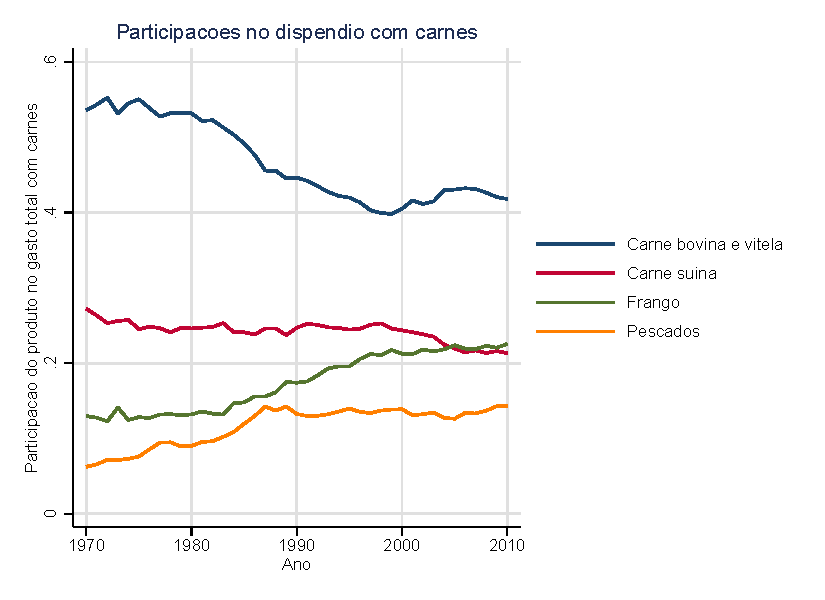
\includegraphics[width=0.92\textwidth]{Figures/Stata/stata_01_participacoes_dispendio.pdf}
    \caption{Participações no dispêndio total com carnes. A figura mostra a evolução de \(w_{\text{bfvl}}\), \(w_{\text{pork}}\), \(w_{\text{poult}}\) e \(w_{\text{fish}}\) ao longo do tempo.}
    \label{fig:participacoes_aids}
\end{figure}

A Figura~\ref{fig:precos_aids} apresenta as séries de preços dos quatro produtos. Como o modelo AIDS identifica respostas de participação a variações de preços relativos, a inspeção das séries de preços é uma etapa preliminar relevante para entender a variação explorada na estimação.

\begin{figure}[H]
    \centering
    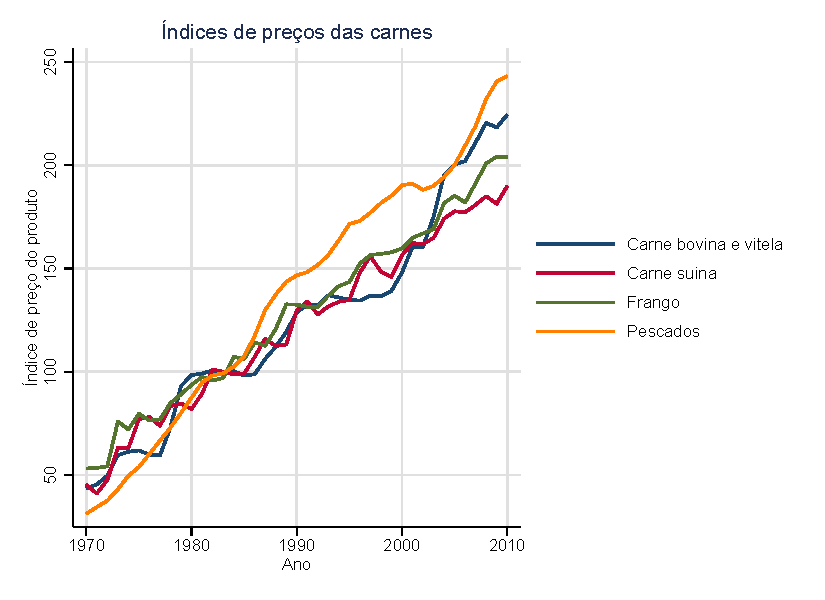
\includegraphics[width=0.92\textwidth]{Figures/Stata/stata_02_precos.pdf}
    \caption{Séries de preços dos produtos incluídos no sistema AIDS.}
    \label{fig:precos_aids}
\end{figure}

A Figura~\ref{fig:lngp_aids} apresenta os log-preços normalizados. Como a média temporal de cada série foi retirada, essas variáveis oscilam em torno de zero. Essa visualização permite verificar a magnitude e a persistência das variações relativas de preço usadas nas equações de demanda.

\begin{figure}[H]
    \centering
    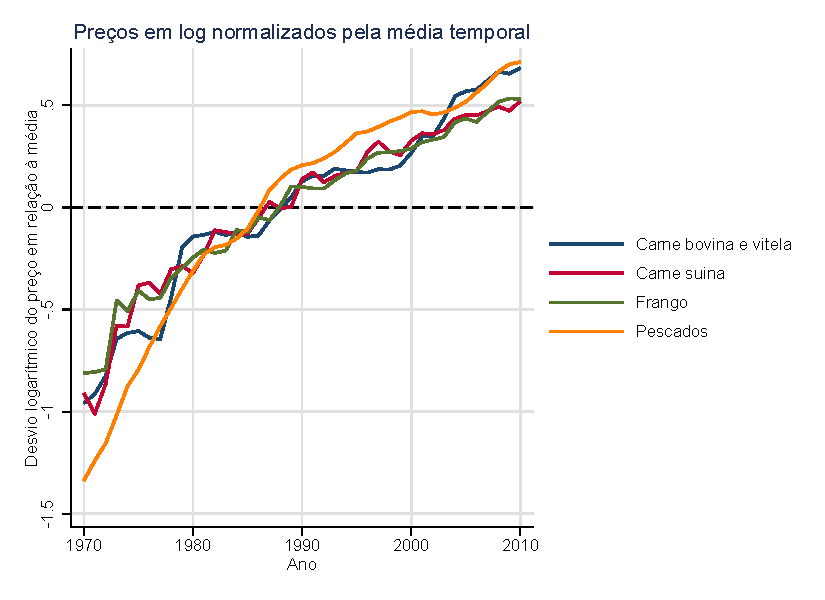
\includegraphics[width=0.92\textwidth]{Figures/Stata/stata_03_log_precos_normalizados.pdf}
    \caption{Log-preços normalizados pela média temporal.}
    \label{fig:lngp_aids}
\end{figure}

A Figura~\ref{fig:stone_real_aids} apresenta o índice de Stone e o dispêndio real com carnes. Essa figura resume a construção da variável de escala do sistema AIDS, definida na equação~\eqref{eq:lnxreal}.

\begin{figure}[H]
    \centering
    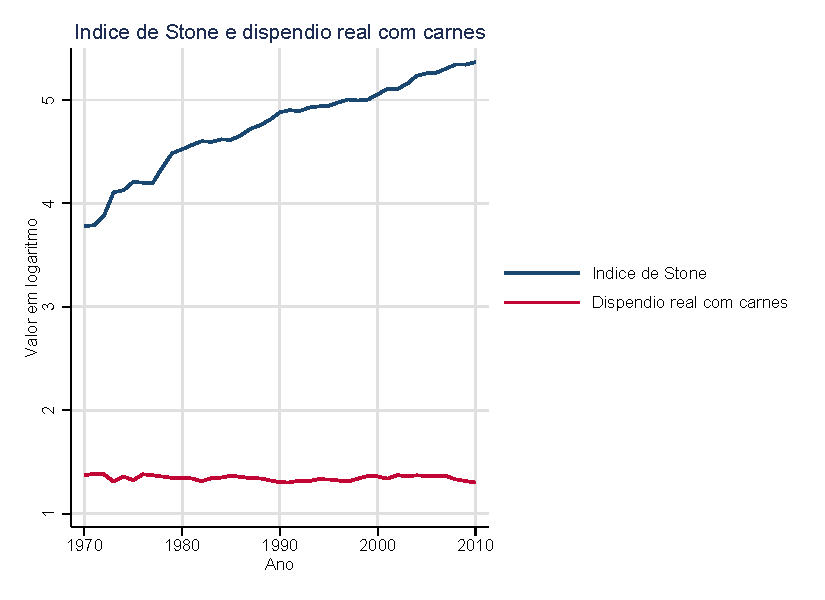
\includegraphics[width=0.92\textwidth]{Figures/Stata/stata_06_stone_dispendio_real.pdf}
    \caption{Índice de Stone e dispêndio real com carnes.}
    \label{fig:stone_real_aids}
\end{figure}

Além dessas figuras principais, a implementação computacional também gera gráficos de checagem da soma das participações, matrizes de dispersão, gráficos observado-versus-previsto, séries de resíduos, histogramas dos resíduos, gráficos de coeficientes, matrizes de elasticidades e diagnósticos da primeira etapa dos instrumentos.

% ================================================================
\section{Implementação Computacional}

A implementação computacional foi realizada nos softwares \textbf{Stata} e \textbf{R}. O Stata foi organizado como a implementação principal, seguindo diretamente a indicação da lista de usar o comando \texttt{gmm} com imposição explícita das restrições por substituição de coeficientes. Em seguida, a implementação em R foi construída como uma tradução da rotina principal, usando GMM linear empilhado e mantendo a mesma lógica de tratamento da base, estimação, recuperação dos parâmetros, cálculo das elasticidades e geração das visualizações.

A estrutura do pacote de replicação foi organizada da seguinte forma:

\begin{verbatim}
pacote_lista_AIDS_2026/
|-- data/
|   |-- raw/                 # base original: meatdata.csv
|   `-- processed/           # bases tratadas
|-- docs/
|   |-- listaDS26.pdf        # enunciado da lista
|   `-- technical_notes.md   # notas técnicas do pacote
|-- output/
|   |-- tables/              # tabelas, matrizes e diagnósticos
|   |-- Figures/Stata/             # gráficos em PDF e PNG
|   |-- logs/                # logs de execução
|   `-- models/              # modelos salvos
|-- stata/                   # scripts .do
`-- R/                       # scripts .R
\end{verbatim}

A execução completa no Stata é feita pelo arquivo:

\begin{verbatim}
stata/run_all_aids_stata.do
\end{verbatim}

Esse script chama, em sequência, todos os arquivos necessários para reproduzir a análise em Stata:

\begin{verbatim}
stata/00_config_aids.do
stata/01_prepare_aids_data.do
stata/02_estimate_aids_stata.do
stata/03_elasticities_aids_stata.do
stata/04_tests_diagnostics_aids_stata.do
stata/05_visualizations_aids_stata.do
\end{verbatim}

O arquivo \texttt{00\_config\_aids.do} define os diretórios globais do projeto. Ele cria os caminhos para a base bruta, bases tratadas, tabelas, figuras, logs e modelos salvos. Essa etapa garante que todos os scripts usem a mesma estrutura de diretórios e que as saídas sejam organizadas de forma replicável.

O tratamento inicial dos dados é realizado por:

\begin{verbatim}
stata/01_prepare_aids_data.do
\end{verbatim}

Esse script importa a base \texttt{meatdata.csv}, declara a dimensão temporal usando a variável \texttt{year} e constrói as variáveis centrais do sistema AIDS. Primeiro, o código calcula ou verifica os dispêndios por produto e soma esses valores para obter o dispêndio total condicional com carnes. Em seguida, calcula as participações \(w_{\text{bfvl}}\), \(w_{\text{pork}}\), \(w_{\text{poult}}\) e \(w_{\text{fish}}\), além da soma anual dessas participações, usada como checagem da restrição de adding-up nos dados. Na sequência, o código calcula os logaritmos dos preços de cada produto e as participações médias \(\bar{w}_g\). Com esses elementos, constrói-se a variável \texttt{lnP\_stone}, definida como a soma ponderada dos log-preços pelos pesos médios de dispêndio, isto é, a implementação direta da Equação~\eqref{eq:stone_expandido}. Depois disso, o script calcula o logaritmo do dispêndio real com carnes conforme a Equação~\eqref{eq:lnxreal}. Essa variável é usada em todas as equações estimadas como o logaritmo do dispêndio real com carnes. Por fim, o script normaliza os log-preços, cria as diferenças de preços usadas para impor homogeneidade e gera as defasagens dos log-preços normalizados, que serão usadas como instrumentos nas estimações por GMM.

As principais saídas dessa etapa são:

\begin{verbatim}
data/processed/meatdata_aids_preparado.dta
data/processed/meatdata_aids_preparado.csv
output/tables/participacoes_medias_stata.csv
\end{verbatim}

A estimação dos modelos é feita pelo script:

\begin{verbatim}
stata/02_estimate_aids_stata.do
\end{verbatim}

Esse arquivo estima três especificações. A primeira é o modelo irrestrito, sem impor homogeneidade e simetria. A segunda é o modelo com homogeneidade. A terceira é o modelo com homogeneidade e simetria. A equação do frango é omitida em todos os casos, mas o frango permanece no cálculo de \(x_t\), de \(\ln P_t^S\), das restrições e das elasticidades.

No modelo irrestrito, as três equações estimadas são:

\[
w_{\text{bfvl},t}
=
\alpha_{\text{bfvl}}
+
\sum_{k \in G}
\gamma_{\text{bfvl},k}lngp_{kt}
+
\beta_{\text{bfvl}}lnxreal_t
+
u_{\text{bfvl},t},
\tag{40}
\label{eq:eq_bfvl_irrestrita}
\]

\[
w_{\text{pork},t}
=
\alpha_{\text{pork}}
+
\sum_{k \in G}
\gamma_{\text{pork},k}lngp_{kt}
+
\beta_{\text{pork}}lnxreal_t
+
u_{\text{pork},t},
\tag{41}
\label{eq:eq_pork_irrestrita}
\]

\[
w_{\text{fish},t}
=
\alpha_{\text{fish}}
+
\sum_{k \in G}
\gamma_{\text{fish},k}lngp_{kt}
+
\beta_{\text{fish}}lnxreal_t
+
u_{\text{fish},t}.
\tag{42}
\label{eq:eq_fish_irrestrita}
\]

No modelo com homogeneidade, os preços entram em diferenças contra o preço do frango, como indicado na equação~\eqref{eq:homog_substituicao}. Assim, para cada equação estimada, o coeficiente de \(lngp_{\text{poult}}\) é recuperado como o negativo da soma dos demais coeficientes de preço.

No modelo com homogeneidade e simetria, além da restrição de soma dos coeficientes de preço dentro de cada equação, impõem-se igualdades entre parâmetros de equações diferentes. Por exemplo:

\[
\gamma_{\text{bfvl},\text{pork}}
=
\gamma_{\text{pork},\text{bfvl}},
\qquad
\gamma_{\text{bfvl},\text{fish}}
=
\gamma_{\text{fish},\text{bfvl}},
\qquad
\gamma_{\text{pork},\text{fish}}
=
\gamma_{\text{fish},\text{pork}}.
\tag{43}
\label{eq:simetria_estimacao}
\]

Os modelos estimados são salvos em:

\begin{verbatim}
output/models/aids_unrestricted.ster
output/models/aids_homogeneity.ster
output/models/aids_hsym.ster
output/models/aids_hsym_L2.ster
\end{verbatim}

As estimativas de coeficientes, erros-padrão e estatísticas \(t\) são salvas inicialmente em arquivos consolidados. Para a apresentação no relatório, esses resultados foram organizados em três tabelas separadas, uma para cada especificação estimada:

\begin{verbatim}
output/tables/coeficientes_stata.dta
output/tables/coeficientes_stata.csv
tables/tab_coeficientes_stata_por_modelo.tex
\end{verbatim}

Após a estimação, o script:

\begin{verbatim}
stata/03_elasticities_aids_stata.do
\end{verbatim}

recupera os parâmetros da equação omitida por adding-up, constrói as matrizes completas de \(\alpha_g\), \(\beta_g\) e \(\gamma_{gk}\), e calcula as elasticidades-dispêndio, elasticidades-preço Marshallianas e elasticidades compensadas.

As principais saídas dessa etapa são:

\begin{verbatim}
output/tables/alpha_hsym_stata.csv
output/tables/beta_hsym_stata.csv
output/tables/gamma_hsym_stata.csv
output/tables/elasticidade_dispendio_hsym_stata.csv
output/tables/elasticidades_marshallianas_hsym_stata.csv
output/tables/elasticidades_compensadas_hsym_stata.csv
\end{verbatim}

A matriz \(\Gamma\), composta pelos parâmetros \(\gamma_{gk}\), é organizada como:

\[
\Gamma
=
\begin{bmatrix}
\gamma_{\text{bfvl},\text{bfvl}} &
\gamma_{\text{bfvl},\text{pork}} &
\gamma_{\text{bfvl},\text{poult}} &
\gamma_{\text{bfvl},\text{fish}} \\

\gamma_{\text{pork},\text{bfvl}} &
\gamma_{\text{pork},\text{pork}} &
\gamma_{\text{pork},\text{poult}} &
\gamma_{\text{pork},\text{fish}} \\

\gamma_{\text{poult},\text{bfvl}} &
\gamma_{\text{poult},\text{pork}} &
\gamma_{\text{poult},\text{poult}} &
\gamma_{\text{poult},\text{fish}} \\

\gamma_{\text{fish},\text{bfvl}} &
\gamma_{\text{fish},\text{pork}} &
\gamma_{\text{fish},\text{poult}} &
\gamma_{\text{fish},\text{fish}}
\end{bmatrix}.
\tag{44}
\label{eq:matriz_gamma}
\]

A matriz de elasticidades Marshallianas é organizada como:

\[
E^M
=
\begin{bmatrix}
\varepsilon^M_{\text{bfvl},\text{bfvl}} &
\varepsilon^M_{\text{bfvl},\text{pork}} &
\varepsilon^M_{\text{bfvl},\text{poult}} &
\varepsilon^M_{\text{bfvl},\text{fish}} \\

\varepsilon^M_{\text{pork},\text{bfvl}} &
\varepsilon^M_{\text{pork},\text{pork}} &
\varepsilon^M_{\text{pork},\text{poult}} &
\varepsilon^M_{\text{pork},\text{fish}} \\

\varepsilon^M_{\text{poult},\text{bfvl}} &
\varepsilon^M_{\text{poult},\text{pork}} &
\varepsilon^M_{\text{poult},\text{poult}} &
\varepsilon^M_{\text{poult},\text{fish}} \\

\varepsilon^M_{\text{fish},\text{bfvl}} &
\varepsilon^M_{\text{fish},\text{pork}} &
\varepsilon^M_{\text{fish},\text{poult}} &
\varepsilon^M_{\text{fish},\text{fish}}
\end{bmatrix}.
\tag{45}
\label{eq:matriz_marshalliana}
\]

A matriz de elasticidades compensadas é organizada de forma análoga:

\[
E^H
=
\left[
\varepsilon^H_{gk}
\right]_{g,k \in G}.
\tag{46}
\label{eq:matriz_hicksiana}
\]

Os testes de restrições e diagnósticos dos instrumentos são realizados pelo script:

\begin{verbatim}
stata/04_tests_diagnostics_aids_stata.do
\end{verbatim}

Esse arquivo compara as três especificações estimadas, executa testes de Wald para as restrições teóricas e organiza estatísticas de comparação entre modelos. A lógica dos testes é avaliar se os dados rejeitam as restrições impostas pela teoria do consumidor.

Para homogeneidade, a hipótese nula é:

\[
H_0^{hom}:
\sum_{k \in G}
\gamma_{gk}
=
0
\quad
\forall g.
\tag{47}
\label{eq:h0_homogeneidade}
\]

Para simetria, a hipótese nula é:

\[
H_0^{sym}:
\gamma_{gk}
=
\gamma_{kg}
\quad
\forall g,k.
\tag{48}
\label{eq:h0_simetria}
\]

A rejeição da homogeneidade indicaria que as participações estimadas respondem a mudanças proporcionais em todos os preços de forma inconsistente com a demanda homogênea de grau zero. Já a rejeição da simetria sugeriria inconsistência com uma estrutura de preferências bem comportada, ao menos dentro da especificação empírica adotada.

As principais saídas dessa etapa são:

\begin{verbatim}
output/tables/testes_wald_restricoes_stata.csv
output/tables/diagnostico_primeira_etapa_stata.csv
output/tables/comparacao_modelos_stata.csv
\end{verbatim}

O diagnóstico de instrumentos é feito por primeira etapa. Para cada preço potencialmente endógeno, estima-se uma regressão do log-preço corrente normalizado contra os instrumentos defasados e os demais regressores exógenos relevantes. O primeiro estágio genérico pode ser escrito como:

\[
lngp_{kt}
=
\pi_{0k}
+
Z_t'\pi_k
+
r_{kt},
\tag{49}
\label{eq:primeira_etapa_aids}
\]

em que \(Z_t\) contém os log-preços normalizados defasados. Para cada preço, reporta-se o teste \(F\) da primeira etapa e o \(R^2\) parcial. O \(R^2\) parcial é calculado como:

\[
R^2_{\text{parcial}}
=
\frac{
R^2_{\text{irrestrito}}
-
R^2_{\text{restrito}}
}
{
1
-
R^2_{\text{restrito}}
}.
\tag{50}
\label{eq:r2_parcial_aids}
\]

O modelo alternativo com segunda defasagem também é estimado para comparar a estabilidade das elasticidades e verificar se a ampliação do conjunto de instrumentos altera substantivamente os resultados.

As visualizações em Stata são geradas pelo script:

\begin{verbatim}
stata/05_visualizations_aids_stata.do
\end{verbatim}

Esse arquivo usa a base tratada, as tabelas de coeficientes, os diagnósticos de instrumentos e as matrizes de elasticidades para construir gráficos em \texttt{PDF} e \texttt{PNG}. As principais figuras geradas são:

\begin{verbatim}
output/Figures/Stata/stata_01_participacoes_dispendio.pdf
output/Figures/Stata/stata_02_precos.pdf
output/Figures/Stata/stata_03_log_precos_normalizados.pdf
output/Figures/Stata/stata_04_dispendios_produto.pdf
output/Figures/Stata/stata_05_dispendio_total_carnes.pdf
output/Figures/Stata/stata_06_stone_dispendio_real.pdf
output/Figures/Stata/stata_07_peso_carnes_pce.pdf
output/Figures/Stata/stata_08_checagem_soma_participacoes.pdf
output/Figures/Stata/stata_09_matriz_dispersao_participacoes.pdf
output/Figures/Stata/stata_10_matriz_dispersao_precos.pdf
output/Figures/Stata/stata_11_observado_previsto_bfvl.pdf
output/Figures/Stata/stata_12_observado_previsto_pork.pdf
output/Figures/Stata/stata_13_observado_previsto_fish.pdf
output/Figures/Stata/stata_14_residuos_series.pdf
output/Figures/Stata/stata_15_hist_residuos_bfvl.pdf
output/Figures/Stata/stata_16_hist_residuos_pork.pdf
output/Figures/Stata/stata_17_hist_residuos_fish.pdf
output/Figures/Stata/stata_18_coeficientes_hsym.pdf
output/Figures/Stata/stata_19_elasticidades_dispendio.pdf
output/Figures/Stata/stata_20_matriz_elasticidades_marshallianas.pdf
output/Figures/Stata/stata_20_matriz_elasticidades_compensadas.pdf
output/Figures/Stata/stata_21_primeira_etapa_F.pdf
output/Figures/Stata/stata_22_primeira_etapa_R2_parcial.pdf
\end{verbatim}

Essas figuras cumprem três funções. Primeiro, permitem descrever os dados antes da estimação, por meio de séries de participações, preços, dispêndios e índice de Stone. Segundo, permitem avaliar os resultados do modelo, por meio de coeficientes, ajustes observado-versus-previsto, resíduos e matrizes de elasticidades. Terceiro, permitem diagnosticar a qualidade dos instrumentos, por meio das estatísticas \(F\) e \(R^2\) parcial da primeira etapa.

Após a implementação em Stata, a análise pode ser reproduzida em R por meio do arquivo:

\begin{verbatim}
R/run_all_aids_R.R
\end{verbatim}

Esse script chama, em sequência:

\begin{verbatim}
R/00_config_aids.R
R/01_prepare_aids_data.R
R/02_estimate_aids_R.R
R/03_elasticities_aids_R.R
R/04_visualizations_aids_R.R
\end{verbatim}

O arquivo \texttt{00\_config\_aids.R} define os caminhos do projeto em R. O arquivo \texttt{01\_prepare\_aids\_data.R} importa a base \texttt{meatdata.csv}, reproduz o tratamento feito no Stata, calcula participações, índice de Stone, dispêndio real, log-preços normalizados e defasagens. As principais saídas dessa etapa são:

\begin{verbatim}
data/processed/meatdata_aids_preparado_R.rds
output/tables/participacoes_medias_R.csv
output/tables/diagnostico_soma_participacoes_R.csv
\end{verbatim}

O arquivo:

\begin{verbatim}
R/02_estimate_aids_R.R
\end{verbatim}

estima os mesmos três modelos do Stata: irrestrito, com homogeneidade e com homogeneidade e simetria. A estimação é feita por uma rotina própria de GMM linear empilhado, sem uso de rotinas prontas de AIDS. As principais saídas são:

\begin{verbatim}
output/tables/coeficientes_R.csv
output/tables/comparacao_modelos_R.csv
output/tables/testes_wald_restricoes_R.csv
output/tables/diagnostico_primeira_etapa_R.csv
output/models/model_unrestricted_R.rds
output/models/model_homogeneity_R.rds
output/models/model_hsym_R.rds
output/models/model_hsym_L2_R.rds
\end{verbatim}

O arquivo:

\begin{verbatim}
R/03_elasticities_aids_R.R
\end{verbatim}

recupera os parâmetros da equação omitida e calcula as mesmas matrizes de elasticidades geradas no Stata. As principais saídas são:

\begin{verbatim}
output/tables/alpha_hsym_R.csv
output/tables/beta_hsym_R.csv
output/tables/gamma_hsym_R.csv
output/tables/gamma_hsym_long_R.csv
output/tables/elasticidade_dispendio_hsym_R.csv
output/tables/elasticidades_marshallianas_hsym_R.csv
output/tables/elasticidades_marshallianas_hsym_long_R.csv
output/tables/elasticidades_compensadas_hsym_R.csv
output/tables/elasticidades_compensadas_hsym_long_R.csv
output/models/elasticidades_hsym_R.rds
\end{verbatim}

Por fim, o arquivo:

\begin{verbatim}
R/04_visualizations_aids_R.R
\end{verbatim}

gera gráficos equivalentes aos do Stata usando \texttt{ggplot2}. As figuras são salvas em \texttt{PDF} e \texttt{PNG}. Entre as principais saídas estão:

\begin{verbatim}
output/Figures/Stata/R_01_participacoes_dispendio.pdf
output/Figures/Stata/R_02_precos.pdf
output/Figures/Stata/R_03_log_precos_normalizados.pdf
output/Figures/Stata/R_04_dispendios_produto.pdf
output/Figures/Stata/R_05_dispendio_total_carnes.pdf
output/Figures/Stata/R_06_stone_dispendio_real.pdf
output/Figures/Stata/R_07_peso_carnes_pce.pdf
output/Figures/Stata/R_08_checagem_soma_participacoes.pdf
output/Figures/Stata/R_09_dispersao_preco_participacao.pdf
output/Figures/Stata/R_13_coeficientes_hsym.pdf
output/Figures/Stata/R_14_estatistica_J_modelos.pdf
output/Figures/Stata/R_15_pvalor_J_modelos.pdf
output/Figures/Stata/R_16_observado_previsto.pdf
output/Figures/Stata/R_17_residuos_series.pdf
output/Figures/Stata/R_18_hist_residuos.pdf
output/Figures/Stata/R_19_residuos_vs_previsto.pdf
output/Figures/Stata/R_20_elasticidades_dispendio.pdf
output/Figures/Stata/R_24_primeira_etapa_F.pdf
output/Figures/Stata/R_25_primeira_etapa_R2_parcial.pdf
output/Figures/Stata/R_26_pvalores_testes_restricoes.pdf
\end{verbatim}

A implementação computacional foi desenhada para garantir replicabilidade e rastreabilidade. Cada etapa da lista possui um script correspondente, e cada resultado empírico é salvo como tabela, matriz, modelo ou figura. O Stata é usado como implementação principal, especialmente por seguir diretamente a recomendação da lista de usar \texttt{gmm}. O R funciona como replicação paralela, permitindo verificar a robustez computacional da rotina, organizar gráficos adicionais e facilitar futuras extensões do exercício.

Assim, a sequência completa da análise é:

\begin{enumerate}[label=(\roman*)]
    \item importar e tratar a base \texttt{meatdata.csv};
    \item calcular dispêndios e participações;
    \item verificar a soma das participações;
    \item calcular o índice de Stone com participações médias;
    \item construir o dispêndio real;
    \item normalizar os log-preços;
    \item criar instrumentos defasados;
    \item estimar o modelo irrestrito;
    \item estimar o modelo com homogeneidade;
    \item estimar o modelo com homogeneidade e simetria;
    \item recuperar a equação omitida do frango por adding-up;
    \item calcular elasticidades-dispêndio;
    \item calcular elasticidades Marshallianas;
    \item calcular elasticidades compensadas;
    \item testar restrições teóricas;
    \item diagnosticar os instrumentos;
    \item comparar especificações com uma e duas defasagens;
    \item gerar tabelas, matrizes e gráficos para interpretação econômica.
\end{enumerate}

Com isso, a implementação procura seguir exatamente a lógica da lista: não usar rotinas prontas de AIDS, impor as restrições diretamente, manter o frango dentro do sistema mesmo com a equação omitida, avaliar elasticidades nas participações médias e apresentar diagnósticos suficientes para discutir tanto a plausibilidade econômica quanto a qualidade econométrica dos resultados.


% ================================================================

% ================================================================
\section{Resultados e Discussão}
% ================================================================

\begin{enumerate}[label=\textbf{\arabic*.}]

% ------------------------------------------------
\item \textbf{Dispêndios e participações no dispêndio.}
Calcule, para cada produto, o dispêndio \(p_{gt}q_{gt}\) e a participação no dispêndio \(w_{gt}\). Verifique numericamente se, em cada período, a soma das participações é igual a um. Caso a soma não seja igual a um, explique o problema de construção da base ou de importação dos dados.

\textbf{Resultados}

A construção do dispêndio segue diretamente da identidade contábil \(p_{gt}q_{gt}\), na qual o preço de cada carne é multiplicado pela quantidade per capita correspondente, conforme a Equação~\eqref{eq:disp_produto}. O dispêndio total com carnes, definido na Equação~\eqref{eq:xtotal}, é obtido pela soma dos quatro dispêndios individuais, e as participações \(w_{gt}\) seguem das Equações~\eqref{eq:w_bfvl_pork} e~\eqref{eq:w_poult_fish}. Como o sistema AIDS é estimado como uma demanda condicional por carnes, o denominador relevante é o gasto total com os quatro produtos do sistema, e não o consumo agregado da economia.

A verificação da identidade \(\sum_{g \in \mathcal{G}}w_{g,t}=1\), expressa na Equação~\eqref{eq:soma_participacoes}, foi feita período a período. Em todos os \(T=41\) anos da amostra, a soma das quatro participações é numericamente igual a um, com erro máximo da ordem de \(10^{-16}\), conforme a Equação~\eqref{eq:erro_soma}. Portanto, as diferenças residuais observadas decorrem apenas de arredondamento numérico de ponto flutuante, e não de erro de construção ou importação da base.


\begin{table}[H]
\centering
\caption{Participações médias no dispêndio por produto}
\label{tab:participacoes-medias}
\small
\begin{tabular}{@{}lcr@{}}
\toprule
Produto & Símbolo & Participação média \\
\midrule
Carne bovina e vitela & $\bar{w}_{\text{bfvl}}$ & 0.4671 \\
Carne suína & $\bar{w}_{\text{pork}}$ & 0.2423 \\
Frango & $\bar{w}_{\text{poult}}$ & 0.1742 \\
Pescados & $\bar{w}_{\text{fish}}$ & 0.1164 \\
\bottomrule
\end{tabular}
\par\vspace{0.35em}
\begin{minipage}{0.92\textwidth}\footnotesize \textit{Nota:} As participações médias $\bar{w}_g$ são usadas como pesos fixos na construção do índice de Stone.\end{minipage}
\end{table}


A Tabela~\ref{tab:participacoes-medias} mostra que carne bovina e vitela respondem, em média, pela maior parcela do dispêndio condicional com carnes, seguidas por carne suína, frango e pescados. Essa hierarquia é importante para todo o restante da lista, pois as participações médias entram diretamente no índice de Stone da Equação~\eqref{eq:stone_media} e também nas fórmulas de elasticidade das Equações~\eqref{eq:elasticidade_dispendio}, \eqref{eq:elasticidade_marshalliana} e~\eqref{eq:elasticidade_hicksiana}. Assim, produtos com maior peso orçamentário, como carne bovina e vitela, tendem a exercer maior influência no deflator específico do sistema de carnes.

\begin{table}[H]
\centering
\caption{Matriz de correlação entre participações no dispêndio}
\label{tab:correlacao-participacoes}
\small
\begin{tabular}{@{}lrrrr@{}}
\toprule
Variável & $\bar{w}_{\text{bfvl}}$ & $\bar{w}_{\text{pork}}$ & $\bar{w}_{\text{poult}}$ & $\bar{w}_{\text{fish}}$ \\
\midrule
$\bar{w}_{\text{bfvl}}$ & 1.0000 & 0.4786 & -0.9476 & -0.9296 \\
$\bar{w}_{\text{pork}}$ & 0.4786 & 1.0000 & -0.6464 & -0.5644 \\
$\bar{w}_{\text{poult}}$ & -0.9476 & -0.6464 & 1.0000 & 0.8314 \\
$\bar{w}_{\text{fish}}$ & -0.9296 & -0.5644 & 0.8314 & 1.0000 \\
\bottomrule
\end{tabular}
\par\vspace{0.35em}
\begin{minipage}{0.92\textwidth}\footnotesize \textit{Nota:} Extraída do arquivo \texttt{matrizes\_correlacao\_stata.xlsx}.\end{minipage}
\end{table}


A Figura~\ref{fig:participacoes_aids} complementa a Tabela~\ref{tab:participacoes-medias} ao mostrar a evolução temporal das participações. Ela evidencia que a composição do dispêndio não permanece fixa ao longo da amostra: há recomposição entre carnes vermelhas, frango e pescados. A Tabela~\ref{tab:correlacao-participacoes} e a Figura~\ref{fig:q1-matriz-dispersao-participacoes} ajudam a interpretar essa recomposição, pois mostram correlações negativas relevantes entre algumas participações. No contexto de um sistema AIDS, esse padrão visual é compatível com deslocamentos de composição do orçamento entre produtos relacionados e antecipa a importância das elasticidades cruzadas discutidas na Questão~7.

\begin{figure}[H]
    \centering
    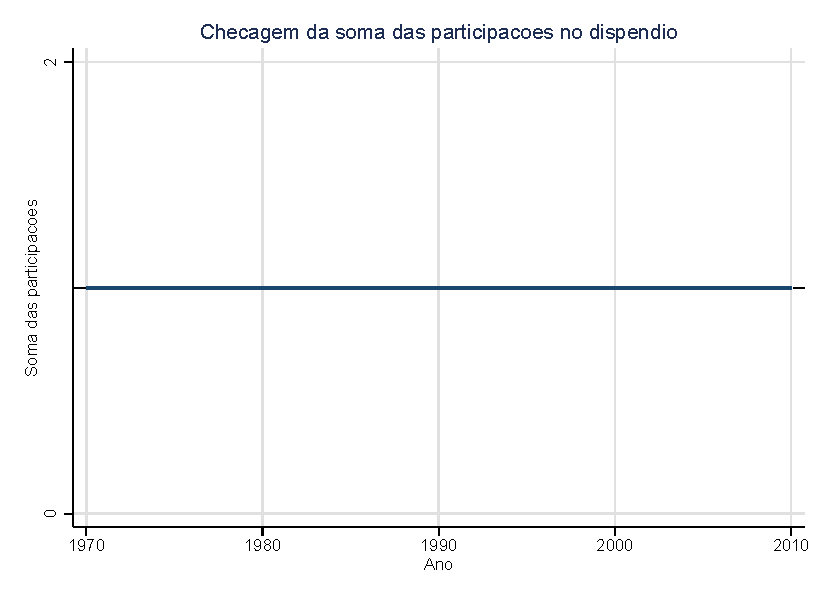
\includegraphics[width=0.85\textwidth]{Figures/Stata/stata_08_checagem_soma_participacoes.pdf}
    \caption{Checagem numérica da soma das participações no dispêndio.}
    \label{fig:q1-checagem-soma-participacoes}
\end{figure}

\begin{figure}[H]
    \centering
    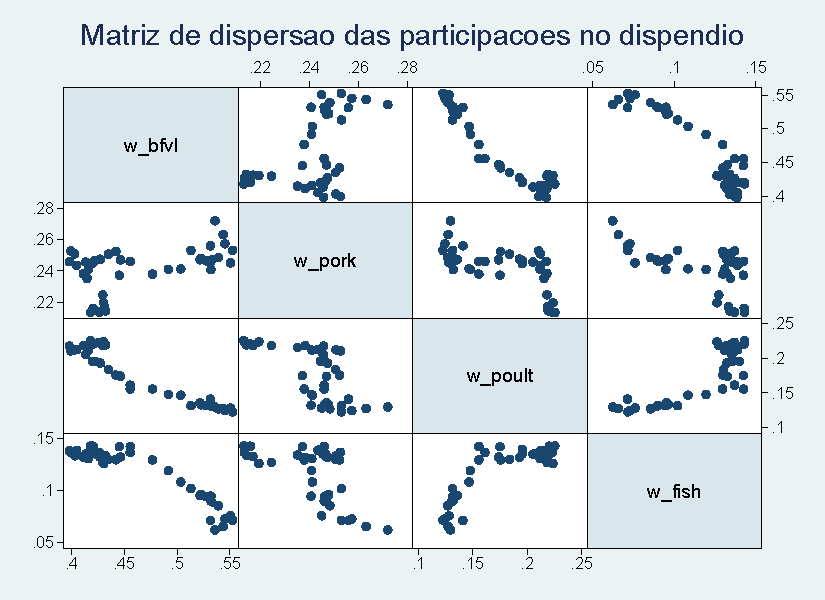
\includegraphics[width=0.80\textwidth]{Figures/Stata/stata_09_matriz_dispersao_participacoes.pdf}
    \caption{Matriz de dispersão das participações no dispêndio.}
    \label{fig:q1-matriz-dispersao-participacoes}
\end{figure}

A Figura~\ref{fig:q1-checagem-soma-participacoes} torna visual o resultado da Equação~\eqref{eq:erro_soma}: a soma das participações permanece sobre a linha de referência igual a um em todos os períodos. Portanto, a base satisfaz a restrição contábil que justifica a omissão de uma equação no sistema. Essa conclusão também sustenta a recuperação posterior dos parâmetros do frango por \textit{adding-up}, conforme as Equações~\eqref{eq:alpha_omitida}, \eqref{eq:beta_omitida} e~\eqref{eq:gamma_omitida}.

% ------------------------------------------------
\item \textbf{Índice de Stone e dispêndio real.}
Calcule o índice de preços de Stone \(\ln P_t^S\) usando as participações médias \(\bar{w}_k\). Em seguida, construa a variável de dispêndio real definida na Equação~\eqref{eq:ln_real_exp}. Explique por que essa variável aparece no sistema AIDS e qual é sua interpretação econômica.

\textbf{Resultados}

O índice de Stone foi calculado com as participações médias reportadas na Tabela~\ref{tab:participacoes-medias}. Como a apostila destaca na apresentação do modelo AIDS, o índice de Stone permite substituir o índice de preços exato do modelo por uma aproximação que não depende dos parâmetros estimados, tornando a equação de participação linear nos parâmetros. Nesta lista, utiliza-se a versão com pesos fixos, dada pela Equação~\eqref{eq:stone_media}, porque ela reduz a correlação mecânica entre a participação contemporânea e o regressor de dispêndio real.

Substituindo as participações médias da Tabela~\ref{tab:participacoes-medias}, obtém-se a expressão operacional:
\begin{equation}
\ln P_t^S
=0{,}4671\ln p_{\text{bfvl},t}
+0{,}2423\ln p_{\text{pork},t}
+0{,}1742\ln p_{\text{poult},t}
+0{,}1164\ln p_{\text{fish},t}.
\label{eq:stone_operacional_resultados}
\end{equation}

A variável de dispêndio real é então construída como \(\ln x_t-\ln P_t^S\), conforme as Equações~\eqref{eq:ln_real_exp} e~\eqref{eq:lnxreal}. Economicamente, esse termo mede a escala real do gasto com carnes. Ele permite separar mudanças na composição do orçamento causadas por preços relativos daquelas associadas ao aumento do dispêndio real total dentro do grupo de carnes. Sem esse deflacionamento, uma elevação generalizada de preços poderia ser interpretada como aumento do gasto real, confundindo efeito preço e efeito dispêndio.

A Tabela~\ref{tab:stone_index} mantém a série temporal usada na construção do índice de Stone e do dispêndio real. Ela explicita que o aumento de \(\ln x_t\) ao longo da amostra combina a evolução nominal do dispêndio e a evolução do índice de preços do grupo de carnes; por isso, a coluna \(\ln(x_t/P_t^S)\) é a medida adequada para interpretar o efeito de escala real no sistema AIDS.

\small
\setlength{\tabcolsep}{4pt}
\renewcommand{\arraystretch}{1.08}

\begin{longtable}{@{}p{0.11\textwidth}rrr@{}}
\caption{Resultados da construção do dispêndio real pelo índice de Stone (1970--2010)}
\label{tab:stone_index}\\
\toprule
Ano 
& {$\ln x_t$} 
& {$\ln P_t^S$} 
& {$\ln(x_t/P_t^S)$} \\
\midrule
\endfirsthead

\multicolumn{4}{c}{\tablename\ \thetable\ -- \textit{continuação}}\\
\toprule
Ano 
& {$\ln x_t$} 
& {$\ln P_t^S$} 
& {$\ln(x_t/P_t^S)$} \\
\midrule
\endhead

\midrule
\multicolumn{4}{r}{\textit{Continua na próxima página...}}\\
\endfoot

\bottomrule
\endlastfoot

1970 & 5,1521 & 3,7799 & 1,3722 \\
1971 & 5,1750 & 3,7891 & 1,3859 \\
1972 & 5,2587 & 3,8782 & 1,3805 \\
1973 & 5,4178 & 4,1069 & 1,3109 \\
1974 & 5,4860 & 4,1263 & 1,3597 \\
1975 & 5,5307 & 4,2067 & 1,3241 \\
1976 & 5,5807 & 4,1999 & 1,3807 \\
1977 & 5,5676 & 4,1965 & 1,3711 \\
1978 & 5,7087 & 4,3497 & 1,3590 \\
1979 & 5,8316 & 4,4856 & 1,3460 \\
1980 & 5,8944 & 4,5345 & 1,3599 \\
1981 & 5,9468 & 4,5575 & 1,3893 \\
1982 & 5,9798 & 4,5786 & 1,4011 \\
1983 & 5,9632 & 4,5770 & 1,3861 \\
1984 & 5,9842 & 4,6114 & 1,3727 \\
1985 & 5,9921 & 4,5864 & 1,4057 \\
1986 & 6,0005 & 4,6063 & 1,3942 \\
1987 & 6,0485 & 4,6460 & 1,4025 \\
1988 & 6,1088 & 4,6752 & 1,4336 \\
1989 & 6,1839 & 4,7261 & 1,4578 \\
1990 & 6,2428 & 4,7690 & 1,4739 \\
1991 & 6,2515 & 4,7782 & 1,4733 \\
1992 & 6,2609 & 4,7619 & 1,4990 \\
1993 & 6,2986 & 4,7920 & 1,5066 \\
1994 & 6,3269 & 4,7717 & 1,5553 \\
1995 & 6,3393 & 4,7731 & 1,5661 \\
1996 & 6,3563 & 4,8079 & 1,5484 \\
1997 & 6,3736 & 4,8197 & 1,5539 \\
1998 & 6,4001 & 4,7917 & 1,6084 \\
1999 & 6,4419 & 4,8029 & 1,6390 \\
2000 & 6,4693 & 4,8511 & 1,6181 \\
2001 & 6,4994 & 4,9047 & 1,5947 \\
2002 & 6,4923 & 4,8740 & 1,6183 \\
2003 & 6,5616 & 4,9644 & 1,5972 \\
2004 & 6,6548 & 5,0675 & 1,5874 \\
2005 & 6,6216 & 5,0767 & 1,5449 \\
2006 & 6,6195 & 5,0585 & 1,5610 \\
2007 & 6,6477 & 5,1022 & 1,5455 \\
2008 & 6,6669 & 5,1455 & 1,5214 \\
2009 & 6,6137 & 5,1048 & 1,5089 \\
2010 & 6,6373 & 5,1342 & 1,5031 \\

\end{longtable}
\normalsize

\begin{figure}[H]
    \centering
    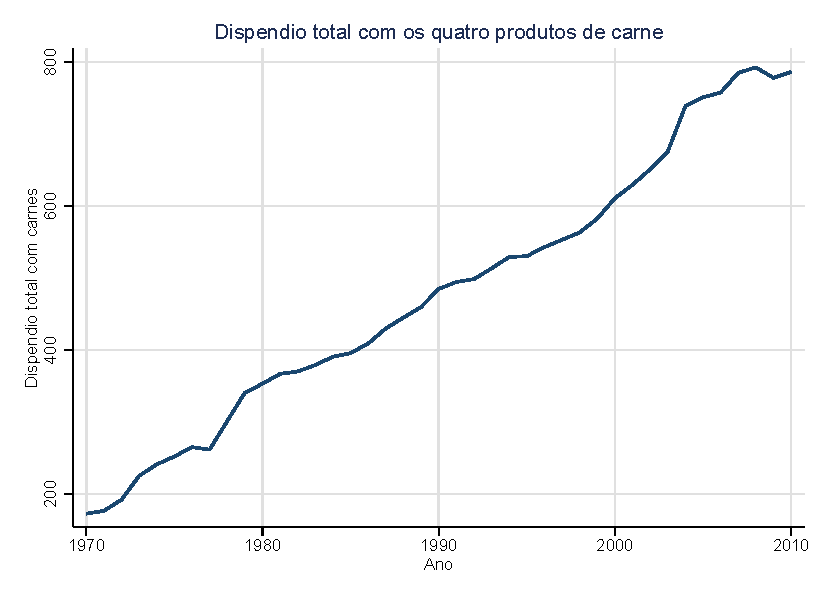
\includegraphics[width=0.88\textwidth]{Figures/Stata/stata_05_dispendio_total_carnes.pdf}
    \caption{Dispêndio total nominal com carnes.}
    \label{fig:q2-dispendio-total-carnes}
\end{figure}

\begin{figure}[H]
    \centering
    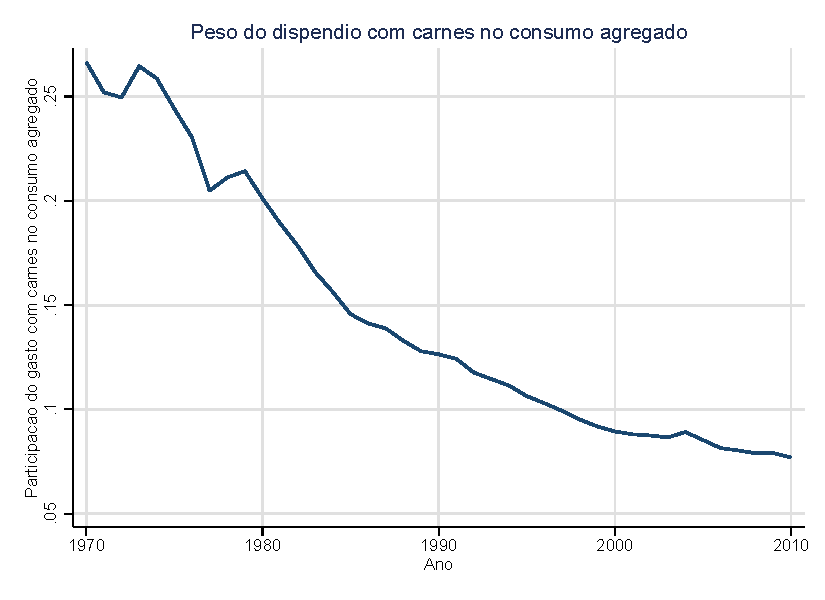
\includegraphics[width=0.82\textwidth]{Figures/Stata/stata_07_peso_carnes_pce.pdf}
    \caption{Peso do dispêndio com carnes no consumo agregado.}
    \label{fig:q2-peso-carnes-pce}
\end{figure}

A Tabela~\ref{tab:stone_index} e a Figura~\ref{fig:stone_real_aids} mostram diretamente a construção do índice de Stone e do dispêndio real. Já a Figura~\ref{fig:q2-dispendio-total-carnes} evidencia a trajetória nominal do gasto com carnes, enquanto a Figura~\ref{fig:q2-peso-carnes-pce} ilustra que esse gasto é apenas uma parcela do consumo agregado. Essa distinção é central: a lista estima uma demanda condicional por carnes, de modo que \(x_t\) deve ser interpretado como o dispêndio total no grupo de carnes, e não como a renda total do consumidor. Por isso, os coeficientes \(\beta_g\), posteriormente apresentados na Tabela~\ref{tab:beta-hsym}, medem como a composição do gasto com carnes muda quando o dispêndio real nesse grupo aumenta.

% ------------------------------------------------
\item \textbf{Normalização dos log-preços.}
Normalize os logaritmos dos preços retirando a média temporal de cada série de preços. Use essas variáveis normalizadas nas equações de demanda. Explique por que a normalização dos log-preços não altera as elasticidades estimadas.

\textbf{Resultados}

A normalização dos log-preços foi feita conforme a Equação~\eqref{eq:normalizacao_precos} e operacionalizada, produto a produto, nas Equações~\eqref{eq:lngp_bfvl}, \eqref{eq:lngp_pork}, \eqref{eq:lngp_poult} e~\eqref{eq:lngp_fish}. Essa transformação apenas desloca a origem de cada série: em vez de usar \(\ln p_{kt}\), usa-se o desvio do log-preço em relação à sua média temporal. Assim, as variações relativas de preço permanecem preservadas.

Como as elasticidades do sistema AIDS dependem dos coeficientes de resposta e das participações médias, e não do nível arbitrário escolhido para a origem dos log-preços, a normalização não altera a interpretação econômica das elasticidades. Sua função é sobretudo econométrica e interpretativa: os interceptos passam a representar participações esperadas quando os log-preços estão em seus valores médios, e a escala dos regressores fica mais bem comportada para a estimação.


\begin{table}[H]
\centering
\caption{Matriz de correlação entre log-preços normalizados}
\label{tab:correlacao-precos}
\small
\begin{tabular}{@{}lrrrr@{}}
\toprule
Símbolo 
& \(lngp_{\text{bfvl},t}\) 
& \(lngp_{\text{pork},t}\) 
& \(lngp_{\text{poult},t}\) 
& \(lngp_{\text{fish},t}\) \\
\midrule
\(lngp_{\text{bfvl},t}\)  & 1.0000 & 0.9735 & 0.9833 & 0.9739 \\
\(lngp_{\text{pork},t}\)  & 0.9735 & 1.0000 & 0.9897 & 0.9861 \\
\(lngp_{\text{poult},t}\) & 0.9833 & 0.9897 & 1.0000 & 0.9842 \\
\(lngp_{\text{fish},t}\)  & 0.9739 & 0.9861 & 0.9842 & 1.0000 \\
\bottomrule
\end{tabular}

\par\vspace{0.35em}
\begin{minipage}{0.92\textwidth}
\footnotesize 
\textit{Nota:} A tabela apresenta as correlações entre os log-preços normalizados usados nas estimações do sistema AIDS.
\end{minipage}
\end{table}


A Figura~\ref{fig:lngp_aids} mostra que as séries normalizadas oscilam em torno de zero, como esperado pela construção da variável. A Tabela~\ref{tab:correlacao-precos} e a Figura~\ref{fig:q3-matriz-dispersao-precos} indicam correlações elevadas entre os log-preços normalizados. Esse resultado é plausível em um mercado de carnes porque os preços dos produtos compartilham componentes comuns de custo, inflação e condições agregadas de oferta. Ao mesmo tempo, essa alta correlação reforça a importância de impor e testar restrições teóricas, pois a identificação dos efeitos cruzados depende de variação relativa suficiente entre os preços.

\begin{figure}[H]
    \centering
    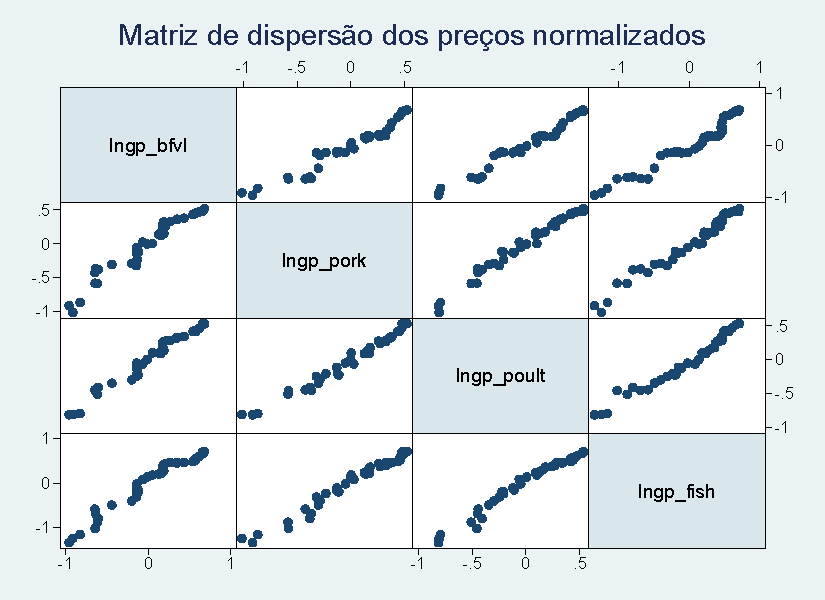
\includegraphics[width=0.80\textwidth]{Figures/Stata/stata_10_matriz_dispersao_precos.pdf}
    \caption{Matriz de dispersão dos log-preços normalizados.}
    \label{fig:q3-matriz-dispersao-precos}
\end{figure}

% ------------------------------------------------
\item \textbf{Estimação do sistema AIDS com omissão da equação do frango.}
Estime o sistema AIDS omitindo a equação do frango. A omissão deve ser entendida como omissão da equação, e não como exclusão do produto do sistema. Use como instrumentos os log-preços defasados em um período, também normalizados pela média amostral, conforme a Equação~\eqref{eq:instrumentos_lag1}. Justifique economicamente o uso de preços defasados como instrumentos para preços correntes.

\textbf{Resultados}

A estimação foi feita a partir da especificação da Equação~\eqref{eq:aids_estimado}, com as três equações observadas para carne bovina e vitela, carne suína e pescados. A equação do frango foi omitida apenas por necessidade econométrica, pois a soma das participações é igual a um, como demonstrado na Figura~\ref{fig:q1-checagem-soma-participacoes}. Portanto, o frango continua no cálculo de \(x_t\), no índice de Stone, nas restrições e nas elasticidades; apenas sua equação não é estimada diretamente.


% ================================================================
% Tabelas de coeficientes AIDS separadas por especificação
% Requer no preâmbulo: \usepackage{booktabs}, \usepackage{float}
% ================================================================

\begin{table}[H]
\centering
\small
\caption{Coeficientes estimados no modelo AIDS irrestrito}
\label{tab:coeficientes-irrestrito}
\begin{tabular}{@{}lrrr@{}}
\toprule
Parâmetro & Estimativa & Erro-padrão & Estatística $t$ \\
\midrule
$\alpha_{\text{bfvl}}$ & 0.4355 & 0.2003 & 2.1749 \\
$\gamma_{\text{bfvl},\text{bfvl}}$ & 0.2502 & 0.0765 & 3.2694 \\
$\gamma_{\text{bfvl},\text{pork}}$ & 0.3608 & 0.1965 & 1.8356 \\
$\gamma_{\text{bfvl},\text{poult}}$ & -0.5682 & 0.2436 & -2.3323 \\
$\gamma_{\text{bfvl},\text{fish}}$ & -0.1652 & 0.0636 & -2.5981 \\
$\beta_{\text{bfvl}}$ & 0.0244 & 0.1490 & 0.1635 \\
$\alpha_{\text{pork}}$ & 0.3855 & 0.0652 & 5.9138 \\
$\gamma_{\text{pork},\text{bfvl}}$ & -0.0531 & 0.0249 & -2.1305 \\
$\gamma_{\text{pork},\text{pork}}$ & 0.0056 & 0.0640 & 0.0879 \\
$\gamma_{\text{pork},\text{poult}}$ & -0.0425 & 0.0793 & -0.5355 \\
$\gamma_{\text{pork},\text{fish}}$ & 0.0488 & 0.0207 & 2.3584 \\
$\beta_{\text{pork}}$ & -0.1068 & 0.0485 & -2.2032 \\
$\alpha_{\text{fish}}$ & 0.1820 & 0.0660 & 2.7578 \\
$\gamma_{\text{fish},\text{bfvl}}$ & -0.0800 & 0.0252 & -3.1698 \\
$\gamma_{\text{fish},\text{pork}}$ & -0.1341 & 0.0648 & -2.0693 \\
$\gamma_{\text{fish},\text{poult}}$ & 0.1163 & 0.0803 & 1.4487 \\
$\gamma_{\text{fish},\text{fish}}$ & 0.1220 & 0.0210 & 5.8213 \\
$\beta_{\text{fish}}$ & -0.0490 & 0.0491 & -0.9975 \\
\bottomrule
\end{tabular}
\par\vspace{0.35em}
\begin{minipage}{0.92\textwidth}
\footnotesize\textit{Nota:} O modelo irrestrito não impõe homogeneidade nem simetria. No sistema AIDS, $\alpha_g$ representa o intercepto da equação de participação do bem $g$; $\gamma_{gk}$ representa o efeito do preço do bem $k$ sobre a participação no dispêndio do bem $g$; e $\beta_g$ representa o efeito do dispêndio real sobre a participação do bem $g$.
\end{minipage}
\end{table}

\begin{table}[H]
\centering
\small
\caption{Coeficientes estimados no modelo AIDS com homogeneidade}
\label{tab:coeficientes-homogeneidade}
\begin{tabular}{@{}lrrr@{}}
\toprule
Parâmetro & Estimativa & Erro-padrão & Estatística $t$ \\
\midrule
$\alpha_{\text{bfvl}}$ & 0.4068 & 0.2360 & 1.7238 \\
$\gamma_{\text{bfvl},\text{bfvl}}$ & 0.1084 & 0.0786 & 1.3804 \\
$\gamma_{\text{bfvl},\text{pork}}$ & 0.2873 & 0.2306 & 1.2457 \\
$\gamma_{\text{bfvl},\text{fish}}$ & -0.3287 & 0.0547 & -6.0058 \\
$\beta_{\text{bfvl}}$ & 0.0460 & 0.1756 & 0.2623 \\
$\alpha_{\text{pork}}$ & 0.3758 & 0.0972 & 3.8671 \\
$\gamma_{\text{pork},\text{bfvl}}$ & -0.1007 & 0.0323 & -3.1119 \\
$\gamma_{\text{pork},\text{pork}}$ & -0.0190 & 0.0950 & -0.2004 \\
$\gamma_{\text{pork},\text{fish}}$ & -0.0061 & 0.0225 & -0.2687 \\
$\beta_{\text{pork}}$ & -0.0996 & 0.0723 & -1.3771 \\
$\alpha_{\text{fish}}$ & 0.1878 & 0.0703 & 2.6693 \\
$\gamma_{\text{fish},\text{bfvl}}$ & -0.0518 & 0.0234 & -2.2114 \\
$\gamma_{\text{fish},\text{pork}}$ & -0.1194 & 0.0687 & -1.7376 \\
$\gamma_{\text{fish},\text{fish}}$ & 0.1545 & 0.0163 & 9.4722 \\
$\beta_{\text{fish}}$ & -0.0533 & 0.0523 & -1.0185 \\
\bottomrule
\end{tabular}
\par\vspace{0.35em}
\begin{minipage}{0.92\textwidth}
\footnotesize\textit{Nota:} A homogeneidade é imposta por diferenças de log-preços contra o preço do frango. Os coeficientes do preço do frango são recuperados pela restrição de soma dos coeficientes de preço. No sistema AIDS, $\alpha_g$ representa o intercepto da equação de participação do bem $g$; $\gamma_{gk}$ representa o efeito do preço do bem $k$ sobre a participação no dispêndio do bem $g$; e $\beta_g$ representa o efeito do dispêndio real sobre a participação do bem $g$.
\end{minipage}
\end{table}

\begin{table}[H]
\centering
\small
\caption{Coeficientes estimados no modelo AIDS com homogeneidade e simetria}
\label{tab:coeficientes-homog-simetria}
\begin{tabular}{@{}lrrr@{}}
\toprule
Parâmetro & Estimativa & Erro-padrão & Estatística $t$ \\
\midrule
$\alpha_{\text{bfvl}}$ & 0.2924 & 0.2728 & 1.0717 \\
$\gamma_{\text{bfvl},\text{bfvl}}$ & -0.1072 & 0.0642 & -1.6690 \\
$\gamma_{\text{bfvl},\text{pork}}=\gamma_{\text{pork},\text{bfvl}}$ & -0.1023 & 0.0325 & -3.1530 \\
$\gamma_{\text{bfvl},\text{fish}}=\gamma_{\text{fish},\text{bfvl}}$ & -0.1495 & 0.0260 & -5.7538 \\
$\beta_{\text{bfvl}}$ & 0.1307 & 0.2030 & 0.6439 \\
$\alpha_{\text{pork}}$ & 0.3757 & 0.0980 & 3.8314 \\
$\gamma_{\text{pork},\text{pork}}$ & -0.0165 & 0.0956 & -0.1729 \\
$\gamma_{\text{pork},\text{fish}}=\gamma_{\text{fish},\text{pork}}$ & -0.0060 & 0.0226 & -0.2635 \\
$\beta_{\text{pork}}$ & -0.0995 & 0.0729 & -1.3634 \\
$\alpha_{\text{fish}}$ & 0.1742 & 0.1470 & 1.1850 \\
$\gamma_{\text{fish},\text{fish}}$ & 0.1679 & 0.0168 & 10.0041 \\
$\beta_{\text{fish}}$ & -0.0433 & 0.1094 & -0.3959 \\
\bottomrule
\end{tabular}
\par\vspace{0.35em}
\begin{minipage}{0.92\textwidth}
\footnotesize\textit{Nota:} Além da homogeneidade, esta especificação impõe simetria entre os efeitos cruzados de preços. Por isso, alguns coeficientes representam simultaneamente dois efeitos cruzados. No sistema AIDS, $\alpha_g$ representa o intercepto da equação de participação do bem $g$; $\gamma_{gk}$ representa o efeito do preço do bem $k$ sobre a participação no dispêndio do bem $g$; e $\beta_g$ representa o efeito do dispêndio real sobre a participação do bem $g$.
\end{minipage}
\end{table}




\begin{table}[H]
\centering
\caption{Parâmetros $\alpha_g$ recuperados no modelo com homogeneidade e simetria}
\label{tab:alpha-hsym}
\small
\begin{tabular}{@{}lr@{}}
\toprule
Parâmetro & Valor \\
\midrule
$\alpha_{\text{bfvl}}$  & 0.2924 \\
$\alpha_{\text{pork}}$  & 0.3757 \\
$\alpha_{\text{poult}}$ & 0.1577 \\
$\alpha_{\text{fish}}$  & 0.1742 \\
\bottomrule
\end{tabular}
\par\vspace{0.35em}
\begin{minipage}{0.92\textwidth}
\footnotesize
\textit{Nota:} Os parâmetros $\alpha_g$ representam os interceptos das equações de participação no dispêndio do bem $g$. Assim, $\alpha_{\text{bfvl}}$, $\alpha_{\text{pork}}$, $\alpha_{\text{poult}}$ e $\alpha_{\text{fish}}$ correspondem, respectivamente, aos interceptos das equações de carne bovina e vitela, carne suína, frango e pescados. O parâmetro do frango é recuperado por \textit{adding-up}, pois sua equação foi omitida na estimação.
\end{minipage}
\end{table}




\begin{table}[H]
\centering
\caption{Parâmetros $\beta_g$ recuperados no modelo com homogeneidade e simetria}
\label{tab:beta-hsym}
\small
\begin{tabular}{@{}lr@{}}
\toprule
Parâmetro & Valor \\
\midrule
$\beta_{\text{bfvl}}$  & 0.1307 \\
$\beta_{\text{pork}}$  & -0.0995 \\
$\beta_{\text{poult}}$ & 0.0120 \\
$\beta_{\text{fish}}$  & -0.0433 \\
\bottomrule
\end{tabular}
\par\vspace{0.35em}
\begin{minipage}{0.92\textwidth}
\footnotesize
\textit{Nota:} Os parâmetros $\beta_g$ medem a resposta da participação no dispêndio do bem $g$ a variações no dispêndio real total com carnes. Assim, $\beta_{\text{bfvl}}$, $\beta_{\text{pork}}$, $\beta_{\text{poult}}$ e $\beta_{\text{fish}}$ correspondem, respectivamente, aos coeficientes de dispêndio real nas equações de carne bovina e vitela, carne suína, frango e pescados. O valor de $\beta_{\text{poult}}$ é recuperado pela restrição de \textit{adding-up}, pois a equação do frango foi omitida na estimação.
\end{minipage}
\end{table}



A Tabela~\ref{tab:coeficientes-irrestrito} apresenta o modelo sem restrições de homogeneidade e simetria. As Tabelas~\ref{tab:coeficientes-homogeneidade} e~\ref{tab:coeficientes-homog-simetria} mostram, respectivamente, as especificações com homogeneidade e com homogeneidade e simetria. Essa organização permite comparar o modelo puramente empírico com versões progressivamente disciplinadas pela teoria do consumidor. As Tabelas~\ref{tab:alpha-hsym} e~\ref{tab:beta-hsym} completam a interpretação ao mostrar os parâmetros recuperados para todos os produtos, inclusive o frango, por meio da restrição de \textit{adding-up}.

A justificativa para usar log-preços defasados como instrumentos vem do problema de endogeneidade de preços discutido na apostila. Em sistemas de demanda, preços correntes podem responder simultaneamente a choques de oferta e de demanda; se esses choques estiverem no termo de erro da equação de participação, a estimação direta fica viesada. Os preços defasados são candidatos a instrumentos porque tendem a ser correlacionados com os preços correntes, por persistência de custos e de condições de mercado, mas são assumidos como não correlacionados com choques contemporâneos não observados de demanda. Essa hipótese de exclusão é econômica e deve ser avaliada com cautela, especialmente em séries com choques persistentes.

\begin{figure}[H]
    \centering
    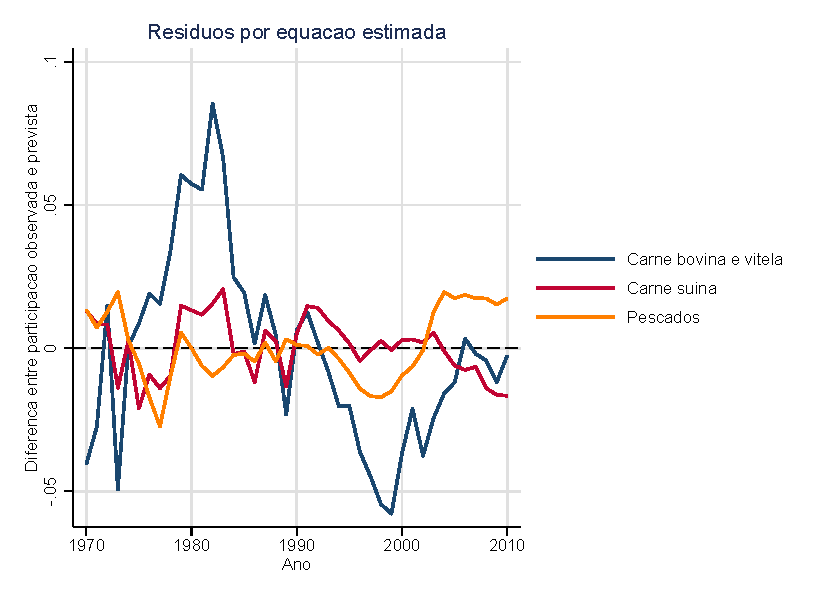
\includegraphics[width=0.92\textwidth]{Figures/Stata/stata_14_residuos_series.pdf}
    \caption{Séries dos resíduos das equações estimadas.}
    \label{fig:q4-residuos-series}
\end{figure}

\begin{figure}[H]
    \centering
    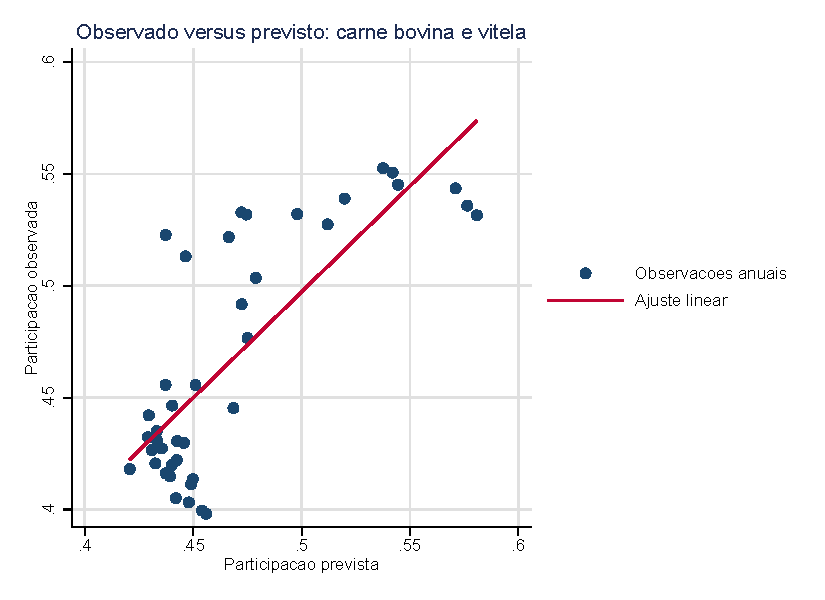
\includegraphics[width=0.78\textwidth]{Figures/Stata/stata_11_observado_previsto_bfvl.pdf}
    \caption{Participação observada e prevista: carne bovina e vitela.}
    \label{fig:q4-observado-previsto-bfvl}
\end{figure}

\begin{figure}[H]
    \centering
    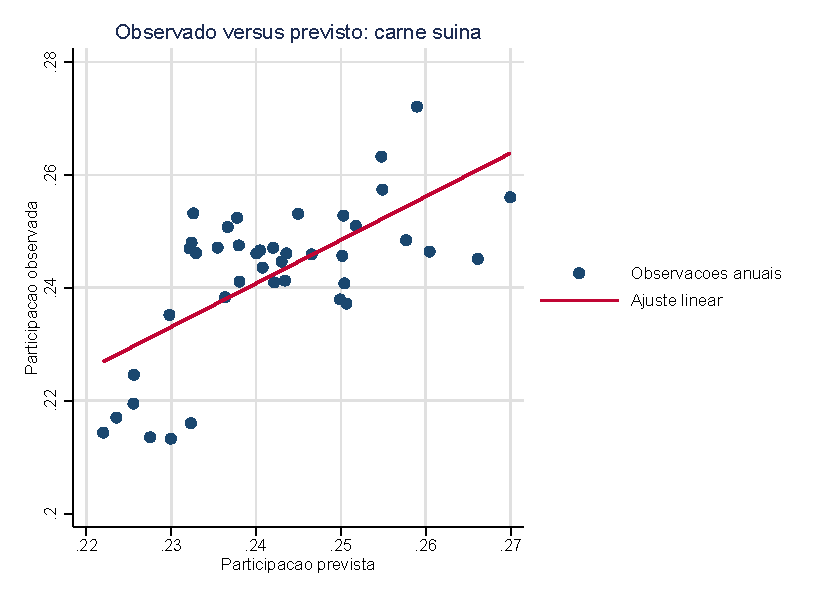
\includegraphics[width=0.78\textwidth]{Figures/Stata/stata_12_observado_previsto_pork.pdf}
    \caption{Participação observada e prevista: carne suína.}
    \label{fig:q4-observado-previsto-pork}
\end{figure}

\begin{figure}[H]
    \centering
    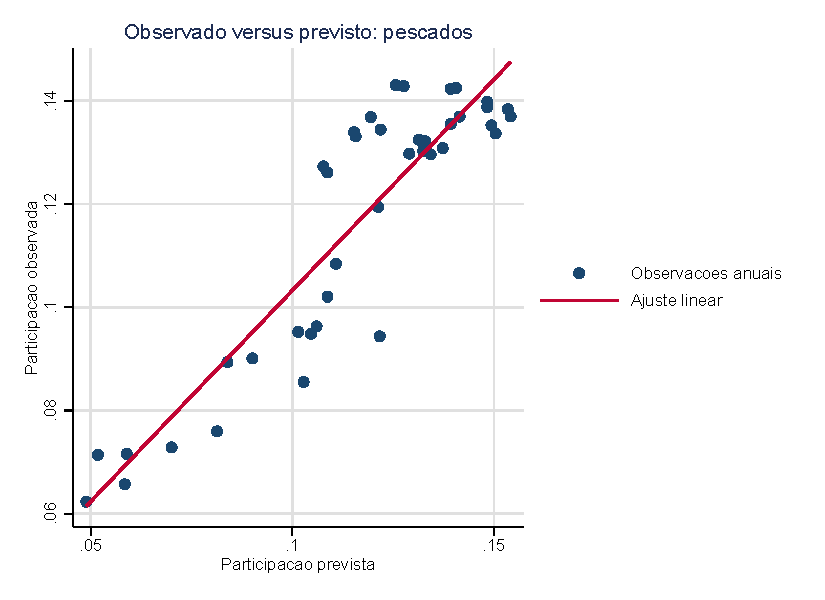
\includegraphics[width=0.78\textwidth]{Figures/Stata/stata_13_observado_previsto_fish.pdf}
    \caption{Participação observada e prevista: pescados.}
    \label{fig:q4-observado-previsto-fish}
\end{figure}

As Figuras~\ref{fig:q4-observado-previsto-bfvl}, \ref{fig:q4-observado-previsto-pork} e~\ref{fig:q4-observado-previsto-fish} mostram que o ajuste acompanha de forma razoável a trajetória das participações observadas nas três equações estimadas. A Figura~\ref{fig:q4-residuos-series} funciona como diagnóstico complementar: resíduos com padrões persistentes sugeririam omissão de variáveis, mudança estrutural ou inadequação das restrições. Assim, as figuras não substituem os testes formais, mas ajudam a interpretar visualmente a qualidade do ajuste que sustenta os resultados das tabelas.

% ------------------------------------------------
\item \textbf{Modelo com homogeneidade.}
Estime inicialmente o sistema impondo a restrição de homogeneidade definida na Equação~\eqref{eq:homogeneidade}. Mostre como substituir um dos coeficientes de preço em cada equação para impor essa restrição diretamente na estimação. Apresente a tabela de coeficientes estimados, erros-padrão e estatísticas \(t\).

\textbf{Resultados}

Pela teoria do consumidor, a homogeneidade de grau zero nos preços e no dispêndio total representa a ausência de ilusão monetária: se todos os preços e o dispêndio nominal aumentam na mesma proporção, as escolhas reais não devem se alterar. No sistema AIDS, isso significa que a soma dos coeficientes de preço dentro de cada equação deve ser nula, como indicado na Equação~\eqref{eq:homogeneidade}.

A imposição direta foi feita por substituição de coeficiente. Tomando o frango como preço de referência, os efeitos de preço em cada equação podem ser escritos em diferenças contra \(lngp_{\text{poult},t}\), conforme a Equação~\eqref{eq:homog_substituicao}. Com isso, o coeficiente associado ao preço do frango é recuperado como o negativo da soma dos demais coeficientes de preço da mesma equação. Essa forma de estimação impõe exatamente a restrição \(\sum_k\gamma_{gk}=0\) e evita estimar um parâmetro redundante.

A Tabela~\ref{tab:coeficientes-homogeneidade} apresenta os coeficientes, erros-padrão e estatísticas \(t\) do modelo com homogeneidade. Em comparação com o modelo irrestrito da Tabela~\ref{tab:coeficientes-irrestrito}, a imposição reduz o número de parâmetros livres e torna a especificação mais alinhada com a teoria. No entanto, ela também desloca alguns coeficientes de preço, especialmente aqueles associados à carne bovina e aos pescados, porque a variação passa a ser interpretada em termos de preços relativos ao frango. Essa mudança é coerente com a própria restrição: o modelo deixa de identificar efeitos de preços nominais isolados e passa a identificar substituições relativas dentro do grupo de carnes.

A comparação com a Tabela~\ref{tab:testes-wald}, discutida na Questão~8, mostra que a homogeneidade é uma restrição teoricamente desejável, mas empiricamente forte nesta base. Portanto, os coeficientes da Tabela~\ref{tab:coeficientes-homogeneidade} devem ser lidos como estimativas disciplinadas pela teoria, não como uma descrição irrestrita dos dados.

% ------------------------------------------------
\item \textbf{Modelo com homogeneidade e simetria.}
Reestime o sistema impondo, além da homogeneidade, a restrição de simetria definida na Equação~\eqref{eq:simetria}. Explique por que essa restrição é uma restrição entre equações. Compare os resultados com o modelo que impõe apenas homogeneidade.

\textbf{Resultados}

A simetria impõe \(\gamma_{gk}=\gamma_{kg}\) para todo par de bens. Diferentemente da homogeneidade, que restringe a soma dos coeficientes de preço dentro de uma mesma equação, a simetria conecta parâmetros que aparecem em equações diferentes. Por exemplo, o efeito do preço da carne suína sobre a participação da carne bovina e vitela deve ser igual ao efeito do preço da carne bovina e vitela sobre a participação da carne suína. Por isso, trata-se de uma restrição entre equações.

A apostila ilustra essa ideia com o exemplo de Coca-Cola e Pepsi: o parâmetro da Pepsi na equação da Coca-Cola deve ser igual ao parâmetro da Coca-Cola na equação da Pepsi. No caso desta lista, a lógica é a mesma, mas aplicada aos produtos de carne. Essa restrição vem da consistência do sistema com uma função de dispêndio e está relacionada à reciprocidade dos efeitos compensados de substituição.

\begin{table}[H]
\centering
\caption{Comparação entre especificações GMM do sistema AIDS}
\label{tab:comparacao-modelos}
\small % <-- Tamanho intermediário
\setlength{\tabcolsep}{6pt} % <-- Espaçamento padrão
\renewcommand{\arraystretch}{1.15} % <-- Altura das linhas moderada
\begin{tabular}{@{}p{7.5cm}rrrrr@{}} % <-- Largura da 1ª coluna ajustada
\toprule
Especificação 
& \(N\) 
& Parâmetros 
& Momentos 
& gl overid. 
& \(J\) \\
\midrule
Modelo sem restrições teóricas
& 40 & 18 & 18 & 0 & 0.0000 \\

Modelo com homogeneidade
& 40 & 15 & 18 & 3 & 14.8150 \\

Modelo com homogeneidade e simetria
& 40 & 12 & 18 & 6 & 36.4051 \\

Modelo com homogeneidade, simetria e instrumentos ampliados
& 39 & 12 & 30 & 18 & 60.8732 \\
\bottomrule
\end{tabular}

\par\vspace{0.35em}
\begin{minipage}{0.95\textwidth} % <-- Minipage com 95% da largura
\scriptsize % <-- Nota ligeiramente menor que a tabela
\textit{Nota:} A coluna \(J\) reporta a estatística de sobreidentificação do GMM. O primeiro modelo é exatamente identificado, pois o número de momentos é igual ao número de parâmetros. Nos demais modelos, as restrições teóricas e/ou a ampliação do conjunto de instrumentos geram graus de liberdade de sobreidentificação.
\end{minipage}
\end{table}


\begin{table}[H]
\centering
\caption{Matriz $\Gamma$ dos efeitos de preços no modelo com homogeneidade e simetria}
\label{tab:gamma-hsym}
\small
\begin{tabular}{@{}lrrrr@{}}
\toprule
Produto demandado & $\gamma_{\cdot,\text{bfvl}}$ & $\gamma_{\cdot,\text{pork}}$ & $\gamma_{\cdot,\text{poult}}$ & $\gamma_{\cdot,\text{fish}}$ \\
\midrule
Carne bovina e vitela & -0.1072 & -0.1023 & 0.3591 & -0.1495 \\
Carne suína & -0.1023 & -0.0165 & 0.1248 & -0.0060 \\
Frango & 0.3591 & 0.1248 & -0.4715 & -0.0124 \\
Pescados & -0.1495 & -0.0060 & -0.0124 & 0.1679 \\
\bottomrule
\end{tabular}
\end{table}


A Tabela~\ref{tab:coeficientes-homog-simetria} apresenta os coeficientes estimados com homogeneidade e simetria, enquanto a Tabela~\ref{tab:gamma-hsym} mostra a matriz completa \(\Gamma\) recuperada para todos os produtos. A simetria fica visível nessa matriz: os elementos fora da diagonal se espelham, como \(\gamma_{\text{bfvl},\text{pork}}=\gamma_{\text{pork},\text{bfvl}}\). A Tabela~\ref{tab:comparacao-modelos} mostra que a imposição adicional reduz o número de parâmetros e aumenta os graus de liberdade de sobreidentificação, tornando a especificação mais parcimoniosa, mas também mais restritiva.

\begin{figure}[H]
    \centering
    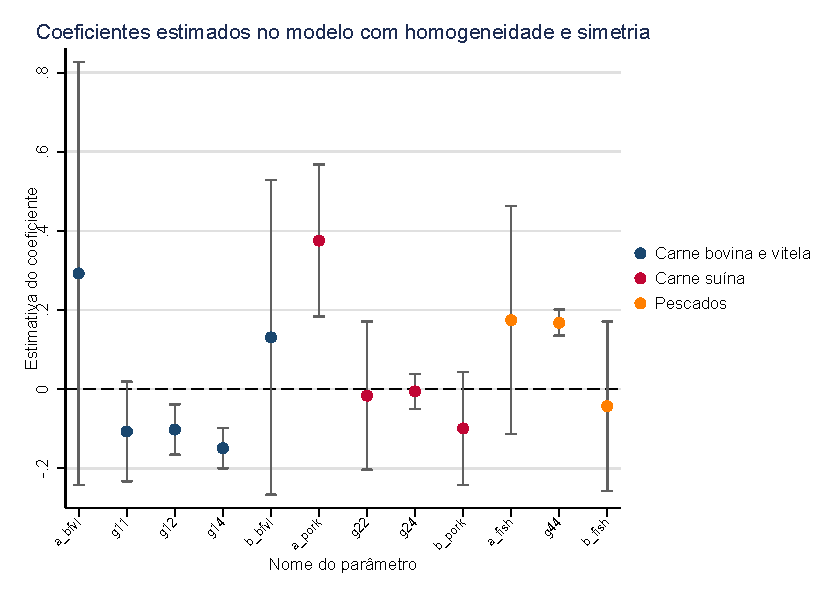
\includegraphics[width=0.92\textwidth]{Figures/Stata/stata_18_coeficientes_hsym.pdf}
    \caption{Coeficientes do modelo com homogeneidade e simetria.}
    \label{fig:q6-coeficientes-hsym}
\end{figure}

A Figura~\ref{fig:q6-coeficientes-hsym} ajuda a visualizar quais parâmetros são mais relevantes no modelo restrito. Em relação ao modelo apenas homogêneo da Tabela~\ref{tab:coeficientes-homogeneidade}, a especificação com simetria reorganiza os efeitos cruzados e força a compatibilidade entre equações. Isso melhora a coerência teórica do sistema, mas pode gerar perda de ajuste caso os dados não sustentem perfeitamente a reciprocidade imposta, ponto avaliado formalmente na Tabela~\ref{tab:testes-wald}.

% ------------------------------------------------
\item \textbf{Elasticidades-dispêndio e elasticidades-preço.}
Com base no modelo estimado, calcule as elasticidades-dispêndio, as elasticidades-preço próprias e as elasticidades-preço cruzadas para todos os produtos. Avalie as elasticidades nas participações médias. Para a versão linear aproximada do AIDS, use a Equação~\eqref{eq:elasticidade_dispendio} para a elasticidade-dispêndio, a Equação~\eqref{eq:elasticidade_marshalliana} para as elasticidades-preço Marshallianas e, se desejar, a Equação~\eqref{eq:elasticidade_hicksiana} para as elasticidades compensadas pela relação de Slutsky. Organize os resultados em uma tabela e discuta se os sinais e magnitudes são economicamente plausíveis.

\textbf{Resultados}

As elasticidades foram calculadas a partir do modelo com homogeneidade e simetria, usando as participações médias da Tabela~\ref{tab:participacoes-medias}. Como a apostila ressalta na discussão do modelo AIDS, os coeficientes \(\gamma_{gk}\) não são elasticidades diretamente interpretáveis. As elasticidades dependem também dos parâmetros \(\beta_g\) e dos pesos de dispêndio \(\bar{w}_g\). Por isso, a Tabela~\ref{tab:gamma-hsym} deve ser lida como insumo intermediário, enquanto as Tabelas~\ref{tab:elasticidade-dispendio}, \ref{tab:elasticidades-marshallianas} e~\ref{tab:elasticidades-compensadas} apresentam os objetos econômicos finais.


\begin{table}[H]
\centering
\caption{Elasticidades-dispêndio avaliadas nas participações médias}
\label{tab:elasticidade-dispendio}
\small
\begin{tabular}{@{}lcr@{}}
\toprule
Produto & Símbolo & Elasticidade \\
\midrule
Carne bovina e vitela & $\eta_{\text{bfvl}}$ & 1.2799 \\
Carne suína & $\eta_{\text{pork}}$ & 0.5896 \\
Frango & $\eta_{\text{poult}}$ & 1.0691 \\
Pescados & $\eta_{\text{fish}}$ & 0.6277 \\
\bottomrule
\end{tabular}
\end{table}


A Tabela~\ref{tab:elasticidade-dispendio} e a Figura~\ref{fig:q7-elasticidades-dispendio} indicam que todos os produtos têm elasticidade-dispêndio positiva. Portanto, dentro do grupo de carnes, todos se comportam como bens normais. Carne bovina e vitela e frango apresentam elasticidades maiores que um, sugerindo resposta mais que proporcional ao aumento do dispêndio real com carnes. Carne suína e pescados têm elasticidades entre zero e um, comportamento mais próximo de bens necessários dentro da cesta.

\begin{figure}[H]
    \centering
    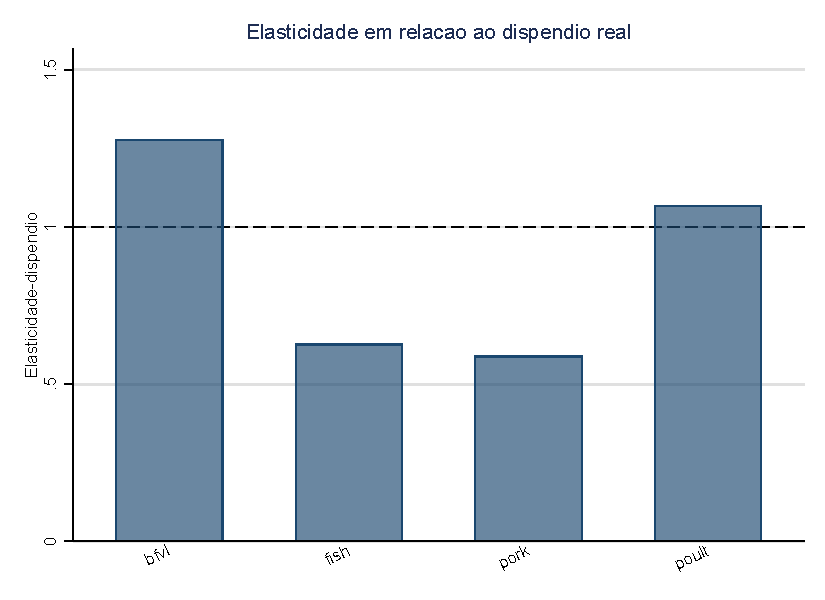
\includegraphics[width=0.82\textwidth]{Figures/Stata/stata_19_elasticidades_dispendio.pdf}
    \caption{Elasticidades em relação ao dispêndio real.}
    \label{fig:q7-elasticidades-dispendio}
\end{figure}

\input{tables/tab_elasticidades_marshallianas_hsym_stata.tex}

A Tabela~\ref{tab:elasticidades-marshallianas} e a Figura~\ref{fig:q7-elasticidades-marshallianas} apresentam as elasticidades-preço Marshallianas, que combinam efeito-substituição e efeito-renda. As elasticidades próprias são negativas para carne bovina e vitela, carne suína e frango, como esperado pela teoria da demanda. A carne bovina e vitela apresenta demanda elástica, a carne suína fica próxima da elasticidade unitária, e o frango tem a maior sensibilidade ao próprio preço. Esses sinais são economicamente plausíveis em um mercado com substitutos próximos.

O resultado menos plausível aparece em pescados, cuja elasticidade própria Marshalliana é positiva. Como a teoria prevê elasticidade própria negativa para uma demanda ordinária bem comportada, esse sinal deve ser interpretado com cautela. Ele pode refletir agregação excessiva da categoria, mudanças de qualidade não observadas, baixa participação média no dispêndio, problemas de mensuração ou instabilidade dos parâmetros.

As elasticidades cruzadas reforçam a leitura de substituição entre algumas carnes. Na Tabela~\ref{tab:elasticidades-marshallianas}, a demanda por carne bovina e vitela responde positivamente ao preço do frango, e a demanda por frango responde positivamente ao preço da carne bovina e vitela. O mesmo ocorre, em menor grau, entre carne suína e frango. Esses padrões são coerentes com a discussão da apostila sobre elasticidade-preço cruzada: sinais positivos indicam substituição, enquanto sinais negativos podem indicar complementaridade ou influência do efeito-renda nas elasticidades Marshallianas.

\begin{figure}[H]
    \centering
    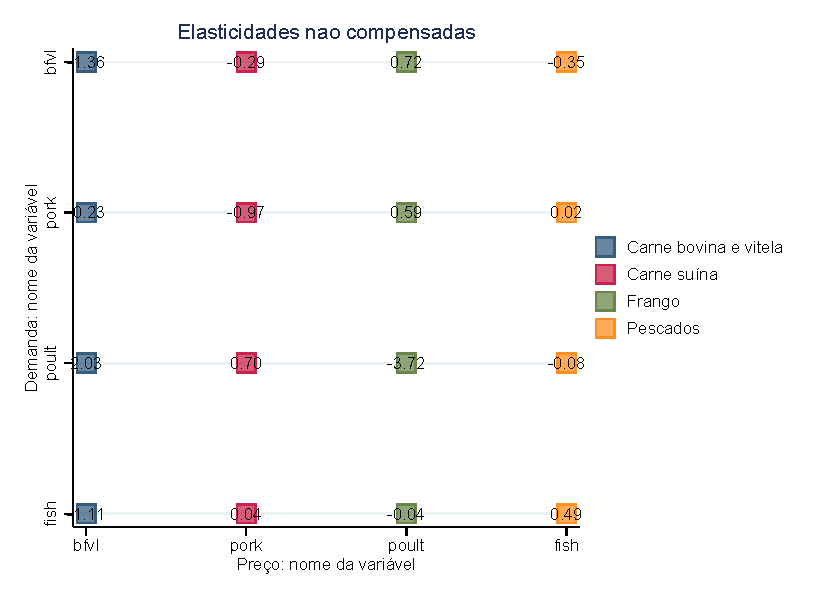
\includegraphics[width=0.82\textwidth]{Figures/Stata/stata_20_matriz_elasticidades_marshallianas.pdf}
    \caption{Matriz de elasticidades-preço Marshallianas.}
    \label{fig:q7-elasticidades-marshallianas}
\end{figure}

\input{tables/tab_elasticidades_compensadas_hsym_stata.tex}

A Tabela~\ref{tab:elasticidades-compensadas} e a Figura~\ref{fig:q7-elasticidades-compensadas} apresentam as elasticidades compensadas, obtidas pela relação de Slutsky da Equação~\eqref{eq:elasticidade_hicksiana}. Como essas elasticidades retiram o efeito-renda, elas se aproximam mais diretamente do efeito-substituição. A comparação com a Tabela~\ref{tab:elasticidades-marshallianas} mostra que a substituição entre carne bovina e vitela, carne suína e frango se torna ainda mais clara na matriz compensada.

Mesmo assim, os problemas de regularidade não desaparecem completamente: a elasticidade própria compensada dos pescados permanece positiva. Portanto, a conclusão é que os resultados são parcialmente plausíveis. As elasticidades-dispêndio têm sinais coerentes, as elasticidades próprias são adequadas para três dos quatro produtos, e as elasticidades cruzadas apontam substituição relevante entre carnes. A exceção dos pescados sugere cautela e ajuda a motivar os testes das restrições teóricas e o diagnóstico de instrumentos nas Questões~8 e~9.

\begin{figure}[H]
    \centering
    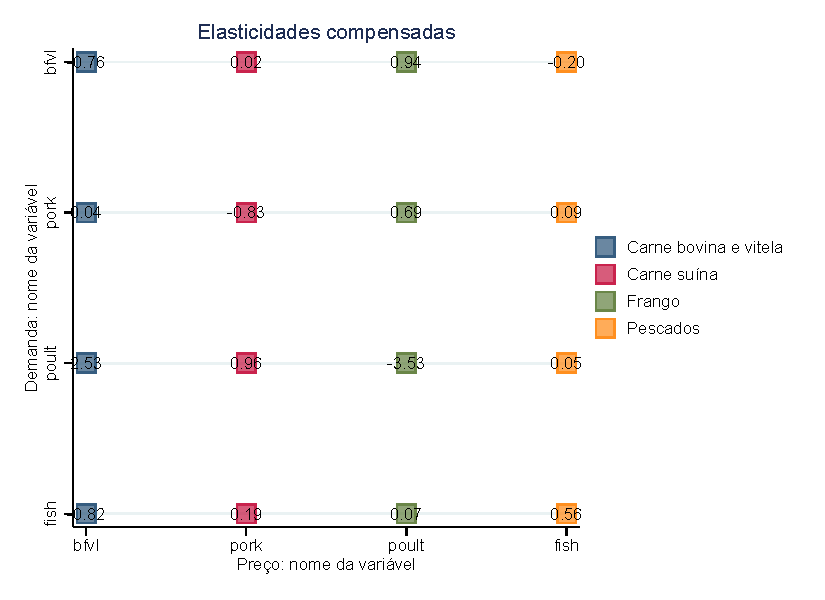
\includegraphics[width=0.82\textwidth]{Figures/Stata/stata_20_matriz_elasticidades_compensadas.pdf}
    \caption{Matriz de elasticidades-preço compensadas.}
    \label{fig:q7-elasticidades-compensadas}
\end{figure}

% ------------------------------------------------
\item \textbf{Testes das restrições teóricas.}
Teste as restrições teóricas do modelo. Estime três especificações: modelo sem impor homogeneidade e simetria, modelo com homogeneidade e modelo com homogeneidade e simetria. Use testes de Wald ou diferenças na estatística objetivo do GMM, quando apropriado, para avaliar se as restrições são rejeitadas pelos dados. Explique a interpretação econômica de rejeitar homogeneidade ou simetria no contexto de demanda por carnes.

\textbf{Resultados}

Foram avaliadas as restrições teóricas do modelo AIDS por meio da comparação entre três especificações: modelo irrestrito, modelo com homogeneidade e modelo com homogeneidade e simetria. Essas restrições derivam da teoria do consumidor aplicada a sistemas de demanda. A aditividade está associada à restrição orçamentária; a homogeneidade indica que apenas preços relativos e dispêndio real devem importar; e a simetria está ligada à consistência dos efeitos de substituição compensados.

\begin{table}[H]
\centering
\caption{Testes de Wald das restrições teóricas}
\label{tab:testes-wald}
\small
\begin{tabular}{@{}lrrr@{}}
\toprule
Teste & Estatística & $g\ell$ & p-valor \\
\midrule
Homogeneidade & 78.2294 & 3 & $7.36\times 10^{-17}$ \\
Simetria & 8.2347 & 3 & 0.0414 \\
\bottomrule
\end{tabular}
\par\vspace{0.35em}
\begin{minipage}{0.92\textwidth}\footnotesize \textit{Nota:} A hipótese nula é a validade da restrição indicada na linha.\end{minipage}
\end{table}


A Tabela~\ref{tab:testes-wald} reporta os testes de Wald. Para a homogeneidade, a estatística é elevada e o p-valor é praticamente zero, levando à rejeição da hipótese nula. Economicamente, isso significa que os dados não sustentam plenamente a ideia de que as participações no dispêndio com carnes dependem apenas de preços relativos e do dispêndio real. Em uma aplicação empírica, essa rejeição pode refletir mudanças de qualidade, agregação de produtos heterogêneos, choques persistentes de oferta ou limitações da aproximação linear do índice de preços.

A simetria também é rejeitada ao nível de \(5\%\), embora com evidência menos forte. Isso sugere que os efeitos cruzados estimados entre produtos não obedecem perfeitamente à reciprocidade esperada pela teoria. Como discutido na Questão~6, essa rejeição não significa simplesmente que duas elasticidades cruzadas são diferentes, pois as elasticidades também dependem das participações médias. Ela indica que a estrutura paramétrica \(\gamma_{gk}=\gamma_{kg}\) não é plenamente compatível com os dados.

A Tabela~\ref{tab:comparacao-modelos} deve ser lida em conjunto com a Tabela~\ref{tab:testes-wald}. A imposição de homogeneidade e simetria aumenta a disciplina teórica e reduz o número de parâmetros, mas também aumenta a estatística objetivo do GMM e os graus de liberdade de sobreidentificação. Essa tensão entre ajuste empírico e coerência teórica é comum em sistemas de demanda. No presente caso, a rejeição das restrições é compatível com os sinais problemáticos observados nas Tabelas~\ref{tab:elasticidades-marshallianas} e~\ref{tab:elasticidades-compensadas}, especialmente na linha dos pescados.

Assim, o modelo com homogeneidade e simetria deve ser interpretado como uma especificação teoricamente disciplinada, útil para organizar as elasticidades, mas não como uma descrição sem tensões empíricas. Os resultados indicam que a teoria do consumidor ajuda a estruturar a estimação, mas a base de carnes apresenta padrões que não se ajustam perfeitamente a todas as restrições do AIDS.

% ------------------------------------------------
\item \textbf{Diagnóstico dos instrumentos.}
Faça um diagnóstico dos instrumentos. Para cada preço potencialmente endógeno, estime a primeira etapa usando os instrumentos defasados e reporte o \(F\) da primeira etapa e o \(R^2\) parcial. Em seguida, estime uma especificação alternativa incluindo também a segunda defasagem dos log-preços como instrumentos. Compare os resultados e discuta se há indícios de instrumentos fracos, excesso de instrumentos ou instabilidade das elasticidades.

\textbf{Resultados}

O diagnóstico dos instrumentos foi feito por regressões de primeira etapa para cada preço potencialmente endógeno. A lógica segue a discussão da apostila sobre variáveis instrumentais: um instrumento válido precisa ser relevante, isto é, correlacionado com o regressor endógeno, e exógeno, isto é, não correlacionado com o erro estrutural da equação de demanda. A primeira etapa avalia diretamente a relevância dos instrumentos, por meio da estatística \(F\) dos instrumentos excluídos e do \(R^2\) parcial.

\begin{table}[H]
\centering
\caption{Diagnóstico de primeira etapa dos instrumentos}
\label{tab:diagnostico-primeira-etapa}
\small
\resizebox{\textwidth}{!}{%
\begin{tabular}{@{}llrrrrrr@{}}
\toprule
Preço & Instrumentos & F excluídos & p-valor & $R^2$ completo & $R^2$ reduzido & $R^2$ parcial & N \\
\midrule
\texttt{bfvl} & \texttt{L1} & 462.55 & $4.03\times 10^{-29}$ & 0.9833 & 0.0724 & 0.9820 & 40 \\
\texttt{pork} & \texttt{L1} & 360.07 & $2.60\times 10^{-27}$ & 0.9788 & 0.0814 & 0.9769 & 40 \\
\texttt{poult} & \texttt{L1} & 358.50 & $2.80\times 10^{-27}$ & 0.9786 & 0.0762 & 0.9768 & 40 \\
\texttt{fish} & \texttt{L1} & 4722.92 & 0.0000 & 0.9983 & 0.0802 & 0.9982 & 40 \\
\texttt{bfvl} & \texttt{L1\_L2} & 252.53 & $1.10\times 10^{-24}$ & 0.9863 & 0.0724 & 0.9853 & 39 \\
\texttt{pork} & \texttt{L1\_L2} & 275.29 & $3.22\times 10^{-25}$ & 0.9875 & 0.0814 & 0.9863 & 39 \\
\texttt{poult} & \texttt{L1\_L2} & 161.61 & $6.21\times 10^{-22}$ & 0.9789 & 0.0762 & 0.9771 & 39 \\
\texttt{fish} & \texttt{L1\_L2} & 2805.65 & 0.0000 & 0.9988 & 0.0802 & 0.9987 & 39 \\
\bottomrule
\end{tabular}%
}
\par\vspace{0.35em}
\begin{minipage}{0.92\textwidth}\footnotesize \textit{Nota:} A especificação \texttt{L1} usa preços defasados em um período; \texttt{L1\_L2} inclui também a segunda defasagem.\end{minipage}
\end{table}


A Tabela~\ref{tab:diagnostico-primeira-etapa} mostra que, usando apenas a primeira defasagem dos log-preços normalizados, as estatísticas \(F\) são muito superiores ao valor de referência usual para instrumentos fracos. Os \(R^2\) parciais também são elevados em todos os preços. Portanto, não há evidência de fraqueza dos instrumentos em termos de relevância. As Figuras~\ref{fig:q9-primeira-etapa-f} e~\ref{fig:q9-primeira-etapa-r2-parcial} resumem visualmente esse resultado: todos os preços apresentam forte poder explicativo na primeira etapa.

\begin{figure}[H]
    \centering
    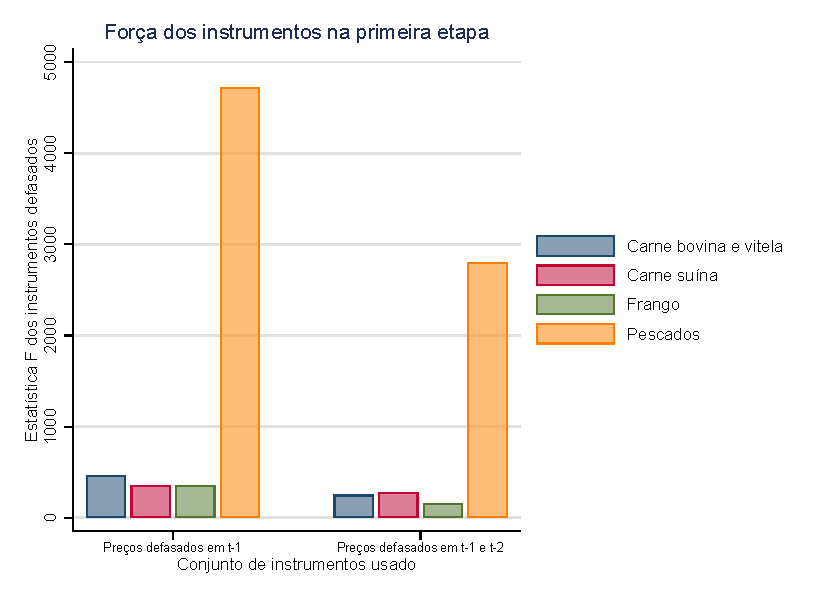
\includegraphics[width=0.86\textwidth]{Figures/Stata/stata_21_primeira_etapa_F.pdf}
    \caption{Estatísticas \(F\) das regressões de primeira etapa.}
    \label{fig:q9-primeira-etapa-f}
\end{figure}

\begin{figure}[H]
    \centering
    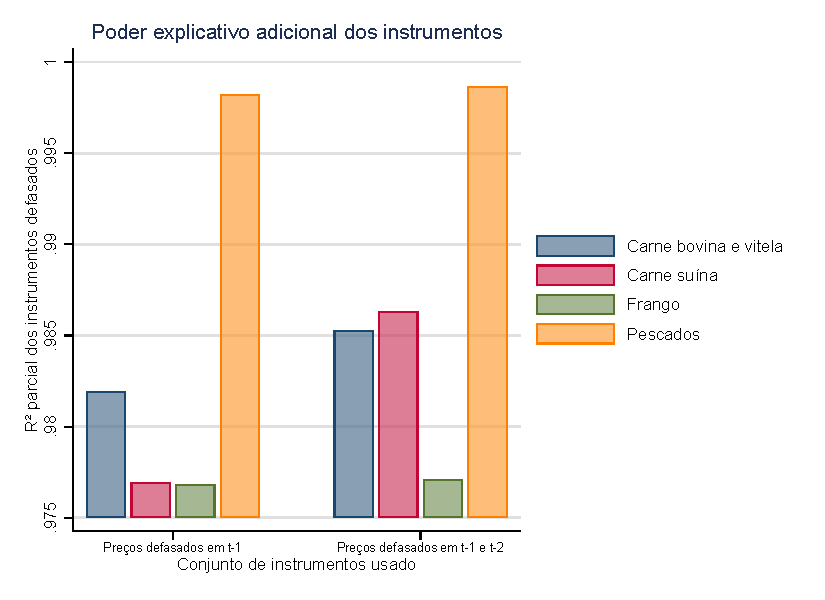
\includegraphics[width=0.86\textwidth]{Figures/Stata/stata_22_primeira_etapa_R2_parcial.pdf}
    \caption{\(R^2\) parcial das regressões de primeira etapa.}
    \label{fig:q9-primeira-etapa-r2-parcial}
\end{figure}

A especificação alternativa com primeira e segunda defasagens também apresenta instrumentos relevantes, mas o ganho é pequeno. Em alguns casos, o \(R^2\) parcial aumenta marginalmente; em outros, a estatística \(F\) cai porque há mais instrumentos e uma observação a menos. Isso não torna a especificação ampliada inadequada, mas sugere cautela. Em GMM, adicionar instrumentos pode aumentar a informação disponível, porém também pode gerar excesso de instrumentos e piorar as propriedades em amostras pequenas.

A Tabela~\ref{tab:comparacao-modelos} reforça esse ponto: o modelo com instrumentos ampliados possui mais momentos e maior grau de sobreidentificação. Assim, a escolha entre \texttt{L1} e \texttt{L1\_L2} deve considerar não apenas a força da primeira etapa, mas também a estabilidade das elasticidades nas Tabelas~\ref{tab:elasticidade-dispendio}, \ref{tab:elasticidades-marshallianas} e~\ref{tab:elasticidades-compensadas}. No conjunto, os instrumentos são fortes quanto à relevância; a principal cautela permanece na hipótese de exogeneidade, pois preços defasados podem carregar choques persistentes de demanda ou de oferta.

\end{enumerate}
\end{document}
